\chapter{\texorpdfstring{\MPI/}{MPI} Environmental Management}
\label{sec:environment}
\label{chap:environment}

This chapter discusses routines for getting and, where appropriate, setting
various parameters that relate to the \MPI/ implementation and the execution environment
(such as error handling).
The procedures for entering and leaving the \MPI/ execution environment are also
described here.

\section{Implementation Information}
\label{sec:inquiry-impl}

\subsection{Version Inquiries}
\mpitermtitleindex{version inquiries}
\label{subsec:inquiry-version}
In order to cope with changes to the \MPI/ standard, there are both compile-time
and run-time ways to determine which version of the standard is in use in the
environment one is using.

The ``version'' will be represented by two separate integers, for the version
and subversion: In C,
%%% Make sure that you also change these values in
%%% chap-appLang/appLang-Const.tex (C preprocessor Constants and Fortran
%%% Parameters)
%%HEADER
%%SKIP
%%ENDHEADER
\begin{lstlisting}[language={[MPI]C}]
#define MPI_VERSION    5
#define MPI_SUBVERSION 0
\end{lstlisting}
in Fortran,
%%HEADER
%%SKIP
%%ENDHEADER
\begin{lstlisting}[language={[MPI]Fortran}]
INTEGER :: MPI_VERSION, MPI_SUBVERSION
PARAMETER (MPI_VERSION    = 5)
PARAMETER (MPI_SUBVERSION = 0)
\end{lstlisting}
\noindent

For runtime determination,

\begin{funcdef}{MPI\_GET\_VERSION}{(\mbox{version}, \mbox{subversion})}
\funcarg{\OUT}{version}{version number (integer)}
\funcarg{\OUT}{subversion}{subversion number (integer)}
\end{funcdef}
\mpibindmain{MPI\_Get\_version}{(\gb{}int~*version, int~*subversion)}
\mpifnewbindmain{MPI\_Get\_version}{(version, subversion, ierror) \fargs INTEGER, INTENT(OUT)\ ::\ \mbox{version}, \mbox{subversion}\fnfinalarg{}INTEGER, OPTIONAL, INTENT(OUT)\ ::\ \mbox{ierror}}
\mpifbindmain{MPI\_GET\_VERSION}{(VERSION, SUBVERSION, IERROR) \fargs \fnfinalarg{}INTEGER \mbox{VERSION}, \mbox{SUBVERSION}, \mbox{IERROR}}

\mpifunc{MPI\_GET\_VERSION} can be called
at any time in an \MPI/ program.
This function must always be thread-safe, as defined in
Section~\ref{sec:ei-threads}\mpitermindex{threads!thread-safe}.
Valid (\mpiconstmain{MPI\_VERSION}, \mpiconstmain{MPI\_SUBVERSION}) pairs in
this and previous versions of the \MPI/ standard
are (5,0), (4,1), (4,0), (3,1), (3,0), (2,2), (2,1), (2,0), and (1,2).

\begin{funcdef}{MPI\_GET\_LIBRARY\_VERSION}{(\mbox{version}, \mbox{resultlen})}
\funcarg{\OUT}{version}{version number (string)}
\funcarg{\OUT}{resultlen}{Length (in printable characters) of the result returned in \mpiarg{version} (integer)}
\end{funcdef}
\mpibindmain{MPI\_Get\_library\_version}{(\gb{}char~*version, int~*resultlen)}
\mpifnewbindmain{MPI\_Get\_library\_version}{(version, resultlen, ierror) \fargs CHARACTER(LEN=MPI\_MAX\_LIBRARY\_VERSION\_STRING), INTENT(OUT)\ ::\ \mbox{version}\fnarg{}INTEGER, INTENT(OUT)\ ::\ \mbox{resultlen}\fnfinalarg{}INTEGER, OPTIONAL, INTENT(OUT)\ ::\ \mbox{ierror}}
\mpifbindmain{MPI\_GET\_LIBRARY\_VERSION}{(VERSION, RESULTLEN, IERROR) \fargs CHARACTER*(*) \mbox{VERSION}\fnfinalarg{}INTEGER \mbox{RESULTLEN}, \mbox{IERROR}}

This routine returns a string representing the version of the \MPI/ library. The version argument is a 
character string for maximum flexibility.

\begin{implementors}
An implementation of \MPI/ should return a different 
string for every change to its source code or build that could be visible 
to the user.
\end{implementors}

The argument \mpiarg{version} must represent storage that is\flushline % fix for margin error
\mpiconstmain{MPI\_MAX\_LIBRARY\_VERSION\_STRING} characters 
long. \mpifunc{MPI\_GET\_LIBRARY\_VERSION} may write up 
to this many characters into \mpiarg{version}.

The number of characters actually written is returned in the 
output argument, \mpiarg{resultlen}. In C, a null character is 
additionally stored at \mpiarg{version[resultlen]}. The value of 
\mpiarg{resultlen} cannot be larger than 
\mpiconst{MPI\_MAX\_LIBRARY\_VERSION\_STRING} - 1. In 
Fortran, \mpiarg{version} is padded on the right with blank characters. 
The value of \mpiarg{resultlen} cannot be larger than 
\mpiconst{MPI\_MAX\_LIBRARY\_VERSION\_STRING}. 

\mpifunc{MPI\_GET\_LIBRARY\_VERSION} can be called
at any time in an \MPI/ program.
This function must always be thread-safe, as defined in
Section~\ref{sec:ei-threads}\mpitermindex{threads!thread-safe}.

\subsection{Environmental Inquiries}
\mpitermtitleindex{environmental inquiries}
\label{subsec:inquiry-inquiry}

When using the \wpm{}\mpitermindex{MPI process initialization@\MPI/ process initialization!\wpm}\mpitermindex{\wpm} (Section~\ref{sec:dynamic:initialization}),
a set of attributes that describe the execution environment is attached to
the communicator \mpiconst{MPI\_COMM\_WORLD} when \MPI/ is initialized.
The values of these attributes can be inquired by using the function
\mpifunc{MPI\_COMM\_GET\_ATTR}
described in 
\sectionref{sec:caching} and in \sectionref{sec:misc-attr}.
It is erroneous to delete these attributes,
free their keys, or change their values.

The list of predefined attribute keys include
\begin{description}
\item[\mpiconstmain{MPI\_TAG\_UB}:]  Upper bound for tag value.
\item[\mpiconstmain{MPI\_IO}:] Rank of an \mpi/ process that has regular I/O facilities (possibly
the rank of the calling \mpi/ process).  \mpi/ processes in the same communicator may return different values for this
parameter.
\item[\mpiconstmain{MPI\_WTIME\_IS\_GLOBAL}:] Boolean variable that indicates
whether clocks are synchronized.
\end{description}

When using the \spm{}\mpitermindex{MPI process initialization@\MPI/ process initialization!\spm}\mpitermindex{\spm} (Section~\ref{sec:model_sessions}),
only the \mpiconst{MPI\_TAG\_UB} attribute is available.
%
Vendors may add implementation-specific parameters (such as node number,
real memory size, virtual memory size, etc.)

These predefined attributes do not change value between \MPI/
initialization (\mpifunc{MPI\_INIT}) and \MPI/ completion
(\mpifunc{MPI\_FINALIZE}), and cannot be updated or deleted by users.

\begin{users}
Note that in the C binding, the value returned by these attributes is a 
\emph{pointer} to an \ctype{int} containing the requested value.
\end{users}

The required parameter values are discussed in more detail below:

\subsubsection{Tag Values}
\mpitermtitleindex{tag values}
Tag values range from \code{0} to the value returned for \mpiconst{MPI\_TAG\_UB},
inclusive.
These values are guaranteed to be unchanging during the execution of an \MPI/
program.
In addition, the tag upper bound value must be \emph{at least} 32767.
An \MPI/ implementation is free to make the value of \mpiconst{MPI\_TAG\_UB} larger
than this;
for example, the value \(2^{30}-1\) is also a valid value for
\mpiconst{MPI\_TAG\_UB}.

In the \spm{}, the attribute \mpiconst{MPI\_TAG\_UB} is attached to
all communicators created by \mpifunc{MPI\_COMM\_CREATE\_FROM\_GROUP} and\flushline
\mpifunc{MPI\_INTERCOMM\_CREATE\_FROM\_GROUPS},
with the same value on all \MPI/ processes in the communicator.
In the \wpm{},
the attribute \mpiconst{MPI\_TAG\_UB} has the same value on all \mpi/ processes
of \mpiconst{MPI\_COMM\_WORLD}.


\subsubsection{IO Rank}
\mpitermtitleindex{IO rank}
The value returned for \mpiconst{MPI\_IO} is the rank of an \mpi/ process that can
provide language-standard I/O facilities.  For Fortran, this means that all of
the Fortran I/O operations are supported (e.g., \code{OPEN}, \code{REWIND},
\code{WRITE}).  For C, 
this means that all of the 
ISO C
I/O operations are
supported (e.g., \code{fopen}, \code{fprintf}, \code{lseek}).

If every \mpi/ process can provide language-standard I/O, then the value
\mpiconst{MPI\_ANY\_SOURCE} will be returned.  Otherwise, if the calling
\mpi/ process can provide language-standard I/O its rank in the group of the communicator will be
returned.  Otherwise, if some \mpi/ process can provide language-standard
I/O then the rank of one such \mpi/ process in the group of the communicator will be returned. The same value
need not be returned by all \mpi/ processes.
If no \mpi/ process can provide
language-standard I/O, then the value
\mpiconst{MPI\_PROC\_NULL} will be  %mansplit
returned.

\begin{users}
Note that input is not collective, and this attribute does \emph{not} indicate
which \mpi/ process can or does provide input.
\end{users}

\subsubsection{Clock Synchronization}
\mpitermtitleindex{clock synchronization}
\label{subsubsec:inquiry-clock-sync}

The value returned for \mpiconst{MPI\_WTIME\_IS\_GLOBAL} is 1 if clocks
at all \mpi/ processes in\flushline % for margin
\mpiconst{MPI\_COMM\_WORLD} are synchronized, 0
otherwise.  A collection of clocks is considered synchronized if
explicit effort has been taken to synchronize them.  The
expectation is that the variation in time, as measured by calls
to \mpifunc{MPI\_WTIME}, will be less then one half the round-trip
time for an \MPI/ message of length zero.  If time is measured at an \mpi/
process just before a send and at another \mpi/ process just after a matching
receive, the second time should be always higher than the first one.

The attribute \mpiconst{MPI\_WTIME\_IS\_GLOBAL} need not be present when
the clocks are not synchronized (however, the attribute key
\mpiconst{MPI\_WTIME\_IS\_GLOBAL} is always valid).
This attribute
may be associated with communicators other then \mpiconst{MPI\_COMM\_WORLD}.

The attribute \mpiconst{MPI\_WTIME\_IS\_GLOBAL} has the same value on all
\mpi/ processes of \mpiconst{MPI\_COMM\_WORLD}.

\subsubsection{Inquire Processor Name}
\mpitermtitleindex{processor name}
\begin{funcdef}{MPI\_GET\_PROCESSOR\_NAME}{(\mbox{name}, \mbox{resultlen})}
\funcarg{\OUT}{name}{A unique specifier for the actual (as opposed to virtual) node.}
\funcarg{\OUT}{resultlen}{Length (in printable characters) of the result returned in \mpiarg{name}}
\end{funcdef}
\mpibindmain{MPI\_Get\_processor\_name}{(\gb{}char~*name, int~*resultlen)}
\mpifnewbindmain{MPI\_Get\_processor\_name}{(name, resultlen, ierror) \fargs CHARACTER(LEN=MPI\_MAX\_PROCESSOR\_NAME), INTENT(OUT)\ ::\ \mbox{name}\fnarg{}INTEGER, INTENT(OUT)\ ::\ \mbox{resultlen}\fnfinalarg{}INTEGER, OPTIONAL, INTENT(OUT)\ ::\ \mbox{ierror}}
\mpifbindmain{MPI\_GET\_PROCESSOR\_NAME}{(NAME, RESULTLEN, IERROR) \fargs CHARACTER*(*) \mbox{NAME}\fnfinalarg{}INTEGER \mbox{RESULTLEN}, \mbox{IERROR}}

This routine returns the name of the processor on which it was called at the
moment of the call.
The name is a character string for maximum flexibility.  From
this value it must be possible to identify a specific piece of hardware;
possible values include ``processor 9 in rack 4 of mpp.cs.org'' and ``231''
(where 231 is the actual processor number in the running homogeneous system).
The argument \mpiarg{name} must represent storage that is at least
\mpiconstmain{MPI\_MAX\_PROCESSOR\_NAME} characters long.
\mpifunc{MPI\_GET\_PROCESSOR\_NAME} may write up to this many characters into
\mpiarg{name}.

The number of characters actually written
is returned in the output argument, \mpiarg{resultlen}.
In C, a null character is additionally stored at \mpiarg{name[resultlen]}.
The value of \mpiarg{resultlen} cannot be larger than \mpiconst{MPI\_MAX\_PROCESSOR\_NAME}-1.
In Fortran, \mpiarg{name} is padded on the right with blank characters.
The value of \mpiarg{resultlen} cannot be larger than \mpiconst{MPI\_MAX\_PROCESSOR\_NAME}.

\begin{rationale}
This function allows \MPI/ implementations that do process
migration to return the current processor.  Note that nothing in \MPI/ 
\emph{requires} or defines process migration; this definition of
\mpifunc{MPI\_GET\_PROCESSOR\_NAME} simply allows such an implementation.
\end{rationale}

\begin{users}
The user must provide at least \mpiconst{MPI\_MAX\_PROCESSOR\_NAME} space
to write the processor name---processor names can be this long.  The user
should examine the 
output 
argument, \mpiarg{resultlen}, to determine
the actual length of the name.
\end{users}

\subsubsection{Inquire Hardware Resource Information}
\label{subsubsec:inquiry-hw-resource-info}
    
\begin{funcdef}{MPI\_GET\_HW\_RESOURCE\_INFO}{(\mbox{hw\_info})}
\funcarg{\OUT}{hw\_info}{info object created (handle)}
\end{funcdef}
\mpibindmain{MPI\_Get\_hw\_resource\_info}{(\gb{}MPI\_Info~*hw\_info)}
\mpifnewbindmain{MPI\_Get\_hw\_resource\_info}{(hw\_info, ierror) \fargs TYPE(MPI\_Info), INTENT(OUT)\ ::\ \mbox{hw\_info}\fnfinalarg{}INTEGER, OPTIONAL, INTENT(OUT)\ ::\ \mbox{ierror}}
\mpifbindmain{MPI\_GET\_HW\_RESOURCE\_INFO}{(HW\_INFO, IERROR) \fargs \fnfinalarg{}INTEGER \mbox{HW\_INFO}, \mbox{IERROR}}

\mpifunc{MPI\_GET\_HW\_RESOURCE\_INFO} is a local procedure that returns an info object containing
information pertaining to the hardware platform on which the calling \MPI/ process is executing at the
moment of the call. This information is stored as (\mpiarg{key},\mpiarg{value})  pairs where each key 
is the name of a hardware resource type and its value is set to \infoval{true} if the calling \MPI/ process
is restricted to a single instance of a hardware resource of that type and \infoval{false} otherwise.
The order in which the keys are stored in  \mpiarg{hw\_info} is unspecified.
This procedure will return different information for \MPI/ processes that are restricted to
different hardware resources. Otherwise, info objects with identical (\mpiarg{key}, \mpiarg{value}) pairs are returned.
The user is responsible for freeing \mpiarg{hw\_info} via \mpifunc{MPI\_INFO\_FREE}.

\begin{users}
  The information returned in the info object might reflect the ``hardware'' resources presented to the application by
  a virtualized environment and may be restricted by access permissions or other constraints like environment
  variables and OS settings.
\end{users}

The keys stored in the \mpiarg{hw\_info} object have a \emph{Uniform Resource Identifier}~(URI) format.
The first part of the URI indicates the key provider and the second part conforms to the format used by
this key provider. The key provider \mpistringmain{mpi://} is reserved for exclusive use by the \MPI/ standard.

\begin{implementors}
  Key provider names could be derived from \MPI/ implementation names (e.g., \mpistringskip{mpich://}, \mpistringskip{openmpi://}),
  from names of external libraries or pieces of software (e.g., \mpistringskip{hwloc://}, \mpistringskip{pmix://}), from names
  of programming or execution models (e.g., \mpistringskip{openmp://}), from resource manager names (e.g., \mpistringskip{slurm://})
  or from hardware vendor names.
\end{implementors}

\begin{users}
  Users should be cautious when using such keys because comparisons between different providers may not be always
  meaningful or relevant. Also, the same hardware resource can be listed by multiple providers under different
  names.
  
\begin{sloppy}  One provider could convey types that represent individual hardware resource instances---for example, \infovalskip{provider\_1://core/FF53C8A9} or \infovalskip{provider\_1://numanode/2}---while another provider could provide types that represent categories or locations of hardware resources{\hspace{0pt}}---for example, \infovalskip{provider\_2://core} or \infovalskip{provider\_2://numanode}.
\end{sloppy}
  
  It is anticipated that types that represent categories
  or locations will be more useful for \mpifunc{MPI\_COMM\_SPLIT\_TYPE}
  than types that represent individual resources.
\end{users}

\begin{users}  
  The keys stored in the info object returned by this procedure can be used in
  \mpifunc{MPI\_COMM\_SPLIT\_TYPE} with the  \mpiarg{split\_type} value  \mpiconst{MPI\_COMM\_TYPE\_HW\_GUIDED}
  or \mpiconst{MPI\_COMM\_TYPE\_RESOURCE\_GUIDED} as key \emph{values} for the info key \infokey{mpi\_hw\_resource\_type}.
\end{users}

Subsequent calls to \mpifunc{MPI\_GET\_HW\_RESOURCE\_INFO} may return different information throughout the execution
of the program because an \MPI/ process can be relocated (e.g., migrated or have its hardware restrictions changed).

\begin{example}
\label{ex:split-with-resrc-info}
\Exindex{C}{Splitting into NUMANode subcommunicators}{MPI\_Get\_hw\_resource\_info,MPI\_Comm\_split\_type}%
 Splitting \mpiconst{MPI\_COMM\_WORLD} into subcommunicators according to
 \gb\mbox{NUMANode} from the hwloc provider.
%%HEADER
%%LANG: C
%%FRAGMENT
%%DECL:#include <string.h>
%%ENDHEADER
\begin{lstlisting}[language={[MPI]C}]
  MPI_Info hw_info;
  MPI_Comm hw_comm;
  int      nb_keys  = 0, flag = 0;
  int      is_found = 0, is_restricted = 0; 
  int      valuelen = 6; // max length between "false" and "true" + 1 
  char    *value    = calloc(valuelen, sizeof(char));
  char    *hw_type  = calloc((MPI_MAX_INFO_KEY+1), sizeof(char));
  
  MPI_Get_hw_resource_info(&hw_info);
  
  MPI_Info_get_nkeys(hw_info, &nb_keys);  
  for(int index = 0 ; index < nb_keys ; index++){
    MPI_Info_get_nthkey(hw_info, index, hw_type);
    MPI_Info_get_string(hw_info, hw_type, &valuelen, value, &flag);     
    if(strcmp(hw_type, "hwloc://NUMANode") == 0){
      is_found = 1;
      if(strcmp(value,"true") == 0)
        is_restricted = 1;
      break; // Resource of type NUMANode found
    }
  }

  // The calling MPI process is restricted to a resource
  // of the chosen type (NUMANode)
  if(is_found  && is_restricted){
    MPI_Info split_info;
    int rank;
    
    MPI_Info_create(&split_info);
    
    // hw_type now serves as value for the "mpi_hw_resource_type" key
    MPI_Info_set(split_info, "mpi_hw_resource_type", hw_type);

    MPI_Comm_rank(MPI_COMM_WORLD, &rank);
    MPI_Comm_split_type(MPI_COMM_WORLD, MPI_COMM_TYPE_RESOURCE_GUIDED,
                        rank, split_info, &hw_comm);

    // Check and use hw_comm from this point if it's a valid
    // communicator or different from MPI_COMM_SELF or MPI_COMM_WORLD.
  } else {
    // If resource is not found or not restricted to it,
    // the calling MPI process does not participate to the call
    // hence the use of MPI_UNDEFINED as split_type and    
    // MPI_COMM_NULL is produced as output communicator
    
    MPI_Comm_split_type(MPI_COMM_WORLD, MPI_UNDEFINED,
                        -1, MPI_INFO_NULL, &hw_comm);       
  }  
\end{lstlisting}
\end{example}

\section{Memory Allocation}
\mpitermtitleindex{memory!allocation}
\label{sec:misc-memalloc}

In some systems, message-passing and remote-memory-access (\RMA/) operations
run faster when accessing specially allocated memory (e.g., memory that is
shared by the other processes in the communicating group on an SMP).  \MPI/
provides a mechanism for allocating and freeing such special memory.  The use
of such memory for message-passing or \RMA/ is not mandatory, and this memory
can be used without restrictions as any other dynamically allocated memory.
However, implementations may restrict the use of some \RMA/ functionality as defined
in Section~\ref{sec:1sided-lock}.

\cdeclindex{MPI\_Info}%
\begin{funcdef}{MPI\_ALLOC\_MEM}{(\mbox{size}, \mbox{info}, \mbox{baseptr})}
\funcarg{\IN}{size}{size of memory segment in bytes (nonnegative integer)}
\funcarg{\IN}{info}{info argument (handle)}
\funcarg{\OUT}{baseptr}{pointer to beginning of memory segment allocated}
\end{funcdef}
\mpibindmain{MPI\_Alloc\_mem}{(\gb{}MPI\_Aint~size, MPI\_Info~info, void~*baseptr)}
\mpifnewbindmain{MPI\_Alloc\_mem}{(size, info, baseptr, ierror) \fargs USE, INTRINSIC\ ::\ ISO\_C\_BINDING, ONLY : C\_PTR \\ INTEGER(KIND=MPI\_ADDRESS\_KIND), INTENT(IN)\ ::\ \mbox{size}\fnarg{}TYPE(MPI\_Info), INTENT(IN)\ ::\ \mbox{info}\fnarg{}TYPE(C\_PTR), INTENT(OUT)\ ::\ \mbox{baseptr}\fnfinalarg{}INTEGER, OPTIONAL, INTENT(OUT)\ ::\ \mbox{ierror}}
\mpifbindmain{MPI\_ALLOC\_MEM}{(SIZE, INFO, BASEPTR, IERROR) \fargs INTEGER(KIND=MPI\_ADDRESS\_KIND) \mbox{SIZE}, \mbox{BASEPTR}\fnfinalarg{}INTEGER \mbox{INFO}, \mbox{IERROR}\mpifoverloadOnlyInAnnex{\>INTERFACE MPI\_ALLOC\_MEM \\ \>\>SUBROUTINE MPI\_ALLOC\_MEM(SIZE, INFO, BASEPTR, IERROR) \\ \>\>\>IMPORT :: MPI\_ADDRESS\_KIND \\ \>\>\>INTEGER :: INFO, IERROR \\ \>\>\>INTEGER(KIND=MPI\_ADDRESS\_KIND) :: SIZE, BASEPTR \\ \>\>END SUBROUTINE \\ \>\>SUBROUTINE MPI\_ALLOC\_MEM\_CPTR(SIZE, INFO, BASEPTR, IERROR) \\ \>\>\>USE, INTRINSIC :: ISO\_C\_BINDING, ONLY : C\_PTR \\ \>\>\>IMPORT :: MPI\_ADDRESS\_KIND \\ \>\>\>INTEGER :: INFO, IERROR \\ \>\>\>INTEGER(KIND=MPI\_ADDRESS\_KIND) :: SIZE \\ \>\>\>TYPE(C\_PTR) :: BASEPTR \\ \>\>END SUBROUTINE \\ \>END INTERFACE}}

If the Fortran compiler provides \ftype{TYPE(C\_PTR)}, 
then the following generic interface must be provided in the \code{mpi}
module and should be provided in the (deprecated) \code{mpif.h} include file through overloading, 
i.e., with the same routine name as the
routine with \mpiftypekind{ADDRESS} \code{BASEPTR}, 
but with a different specific procedure name:

%%HEADER
%%SKIP
%%ENDHEADER
\begin{verbatim}
INTERFACE MPI_ALLOC_MEM
    SUBROUTINE MPI_ALLOC_MEM(SIZE, INFO, BASEPTR, IERROR)
        IMPORT :: MPI_ADDRESS_KIND
        INTEGER :: INFO, IERROR
        INTEGER(KIND=MPI_ADDRESS_KIND) :: SIZE, BASEPTR
    END SUBROUTINE
    SUBROUTINE MPI_ALLOC_MEM_CPTR(SIZE, INFO, BASEPTR, IERROR)
        USE, INTRINSIC :: ISO_C_BINDING, ONLY : C_PTR
        IMPORT :: MPI_ADDRESS_KIND
        INTEGER :: INFO, IERROR
        INTEGER(KIND=MPI_ADDRESS_KIND) :: SIZE
        TYPE(C_PTR) :: BASEPTR
    END SUBROUTINE
END INTERFACE
\end{verbatim}
 
The base procedure name of this overloaded function is \mpifuncmain{MPI\_ALLOC\_MEM\_CPTR}. The implied specific procedure names
are described in \sectionref{sec:f90:linker-names}.

\mpitermindex{memory!alignment}\mpitermindex{alignment}
By default, the allocated memory shall be aligned to at least the alignment
required for load/store accesses of any datatype corresponding to a
predefined \MPI/ datatype.
%
The \mpiarg{info} argument may be used to specify a desired alternative minimum alignment in bytes for the
allocated memory by setting the value of the key \infokeymain{mpi\_minimum\_memory\_alignment} to an integral number
equal to a power of two.
An implementation may ignore values smaller than the default required alignment.
The \mpiarg{info} argument can also be used to provide
directives that control the desired location of the allocated memory.
Such a directive does not affect the semantics of the call.
The corresponding \mpiarg{info} values are
implementation-dependent. A null directive value of
\mpiarg{info}\mpicode{ = }\mpiconst{MPI\_INFO\_NULL} is always valid.

The  function \mpifunc{MPI\_ALLOC\_MEM} may raise an error of class
\errormain{MPI\_ERR\_NO\_MEM} 
to indicate it failed because memory 
is exhausted.

\begin{funcdef}{MPI\_FREE\_MEM}{(\mbox{base})}
\funcarg{\IN}{base}{initial address of memory segment allocated by \mpifunc{MPI\_ALLOC\_MEM} (choice)}
\end{funcdef}
\mpibindmain{MPI\_Free\_mem}{(\gb{}void~*base)}
\mpifnewbindmain{MPI\_Free\_mem}{(base, ierror) \fargs TYPE(*), DIMENSION(..), INTENT(IN), ASYNCHRONOUS\ ::\ \mbox{base}\fnfinalarg{}INTEGER, OPTIONAL, INTENT(OUT)\ ::\ \mbox{ierror}}
\mpifbindmain{MPI\_FREE\_MEM}{(BASE, IERROR) \fargs <type> \mbox{BASE(*)}\fnfinalarg{}INTEGER \mbox{IERROR}}

The function \mpifunc{MPI\_FREE\_MEM} may raise an error of class
\errormain{MPI\_ERR\_BASE} to indicate an invalid base argument.

\begin{rationale}
The C bindings of \mpifunc{MPI\_ALLOC\_MEM} and
\mpifunc{MPI\_FREE\_MEM} are similar to the bindings for the
\code{malloc} and \code{free} C library calls:
a call to
\cfunc{MPI\_Alloc\_mem($\ldots$, \&base)} should be paired with a call to
\cfunc{MPI\_Free\_mem(base)} (one less 
level of indirection). Both arguments are declared to
be of same type \code{void*} so as to facilitate type casting.
The Fortran binding is consistent with the C bindings:
the Fortran \mpifunc{MPI\_ALLOC\_MEM} call returns in 
\mpiarg{baseptr} the \ftype{TYPE(C\_PTR)} pointer or
the (integer valued) address 
of the allocated memory.
The \mpiarg{base} argument of \mpifunc{MPI\_FREE\_MEM} is a choice
argument, which passes (a reference to) the variable stored at that location.
\end{rationale}

\begin{implementors}
If \mpifunc{MPI\_ALLOC\_MEM} allocates special memory, then
a design similar to the design of C \code{malloc} and \code{free}
functions has to
be used, in order to find out the size of a memory segment, when the segment is freed.
If no special memory is used,
\mpifunc{MPI\_ALLOC\_MEM} simply invokes \code{malloc}, and \mpifunc{MPI\_FREE\_MEM} invokes \code{free}.

A call to \mpifunc{MPI\_ALLOC\_MEM} can be used in shared memory
systems to allocate  memory in a shared memory segment.
\end{implementors}

\begin{example}
\label{ex:1side-fmalloc-ptr}
\Exindex{Fortran}{Use of Alloc\_mem in Fortran}{MPI\_Alloc\_mem,MPI\_Free\_mem}%
Example use of \mpifunc{MPI\_ALLOC\_MEM} in Fortran with
\ftype{TYPE(C\_PTR)} pointers. We assume 4-byte \ftype{REAL}s.
%%HEADER
%%LANG: FORTRAN08
%%FRAGMENT
%%NOADDMPIMOD
%%DECLAFTERMOD: INTEGER:: ierr
%%NOIMPLICITNONE
%%SKIPELIPSIS
%%ENDHEADER
\begin{lstlisting}[language={[MPI08]Fortran},basicstyle=\lstsmall]
USE mpi_f08   !  or  USE mpi      (not guaranteed with INCLUDE 'mpif.h')
USE, INTRINSIC :: ISO_C_BINDING
TYPE(C_PTR) :: p
REAL, DIMENSION(:,:), POINTER :: a            ! no memory is allocated
INTEGER, DIMENSION(2) :: shape
INTEGER(KIND=MPI_ADDRESS_KIND) :: size
shape = (/100,100/)
size = 4 * shape(1) * shape(2)                ! assuming 4 bytes per REAL
CALL MPI_ALLOC_MEM(size,MPI_INFO_NULL,p,ierr) ! memory is allocated and
CALL C_F_POINTER(p, a, shape) ! intrinsic     ! now accessible via a(i,j)
...                           ! in ISO_C_BINDING
a(3,5) = 2.71
...
CALL MPI_FREE_MEM(a, ierr)                    ! memory is freed
\end{lstlisting}
\end{example}

\begin{example}
\label{ex:1side-fmalloc}
\Exindex{Fortran}{Use of Alloc\_mem in Fortran with Cray
  pointers}{MPI\_Alloc\_mem,MPI\_Free\_mem}%
Example use of \mpifunc{MPI\_ALLOC\_MEM} in Fortran with
nonstandard \mpitermdef{Cray-pointers}.
We assume 4-byte \ftype{REAL}s, and assume that these pointers
are address-sized.
%%HEADER
%%LANG: FORTRAN
%%EXTRAFLAGS:pointer
%%FRAGMENT
%%SKIPELIPSIS
%%DECL: integer IERR
%%ENDHEADER
\begin{lstlisting}[language={[MPI]Fortran}]
REAL A
POINTER (P, A(100,100))   ! no memory is allocated
INTEGER(KIND=MPI_ADDRESS_KIND) SIZE
SIZE = 4*100*100
CALL MPI_ALLOC_MEM(SIZE, MPI_INFO_NULL, P, IERR)
! memory is allocated
...
A(3,5) = 2.71
...
CALL MPI_FREE_MEM(A, IERR) ! memory is freed
\end{lstlisting}

This code is not Fortran 77 or Fortran 90 code.
Some compilers 
may 
not support this code or need a special option, e.g., the GNU gFortran compiler needs \code{-fcray-pointer}.

\begin{implementors}
Some compilers map Cray-pointers to address-sized integers,
some to \ftype{TYPE(C\_PTR)} pointers (e.g., Cray Fortran, version 7.3.3).
From the user's viewpoint, this mapping is irrelevant 
because Examples~\ref{ex:1side-fmalloc} should work correctly with
an \MPIIIIDOTO/ (or later) library if Cray-pointers are available. 
\end{implementors}
\end{example}

\begin{example}
\Exindex{C}{Using Alloc\_mem}{MPI\_Alloc\_mem}%
Same example, in C.
%%HEADER
%%LANG: C
%%FRAGMENT
%%SKIPELIPSIS
%%ENDHEADER
\begin{lstlisting}[language={[MPI]C}]
float  (* f)[100][100];
/* no memory is allocated */
MPI_Alloc_mem(sizeof(float)*100*100, MPI_INFO_NULL, &f);
/* memory allocated */
...
(*f)[5][3] = 2.71;
...
MPI_Free_mem(f);
\end{lstlisting}
\end{example}

\section{Error Handling}
\mpitermtitleindex{error handling}
\label{sec:errorhandler}

An \MPI/ implementation may be unable or choose not to handle some failures
that occur during \MPI/ calls.  These can include failures that generate
exceptions or traps, such as floating point errors or access
violations.
The set of failures that are handled by \MPI/ is implementation-dependent.
Each such failure causes an error to be raised.

The above text takes precedence over any text on error handling within this
document.  Specifically, text that states that errors \emph{will} be handled
should be read as \emph{may} be handled.
More background information about how \MPI/ treats errors can be found in
Section~\ref{sec:terms-errorhandling}.

\begin{figure}
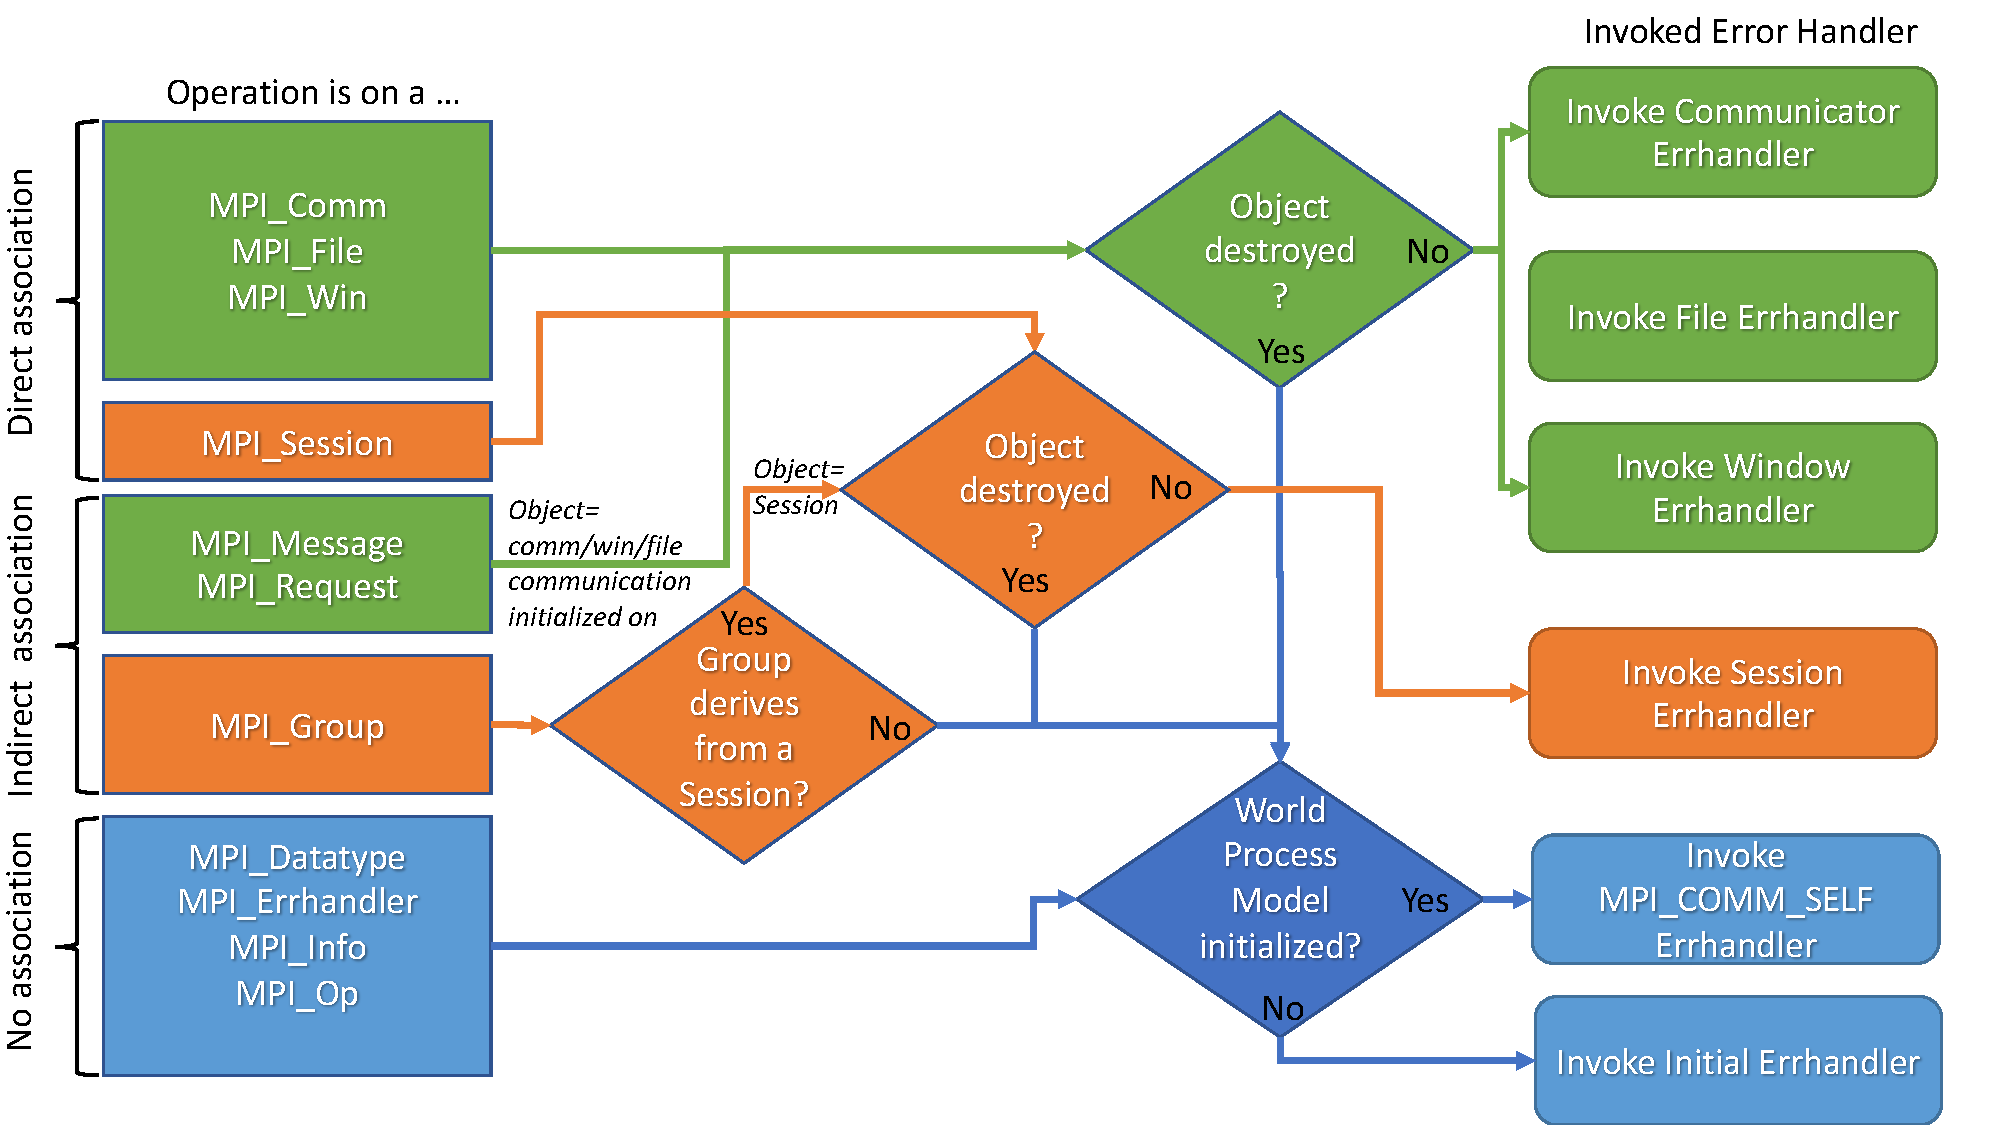
\includegraphics[width=6in]{figures/errh-fallback-figure}
\caption{Diagram for deciding which error handler is invoked depending on the \MPI/ objects associated with the operation and whether the \spm{} or the \wpm{} is used.}
\label{fig:errhandler:fallback}
\end{figure}

A user can associate error handlers to four types of objects:
communicators, windows, files, and sessions.  The
specified error handling routine will be used for any error
that occurs during an \MPI/ procedure or an operation that refers to
the respective object.
%
Figure~\ref{fig:errhandler:fallback}
presents a diagram of the error handler that is invoked in different situations.
When the \MPI/ procedure or operation refers to a communicator, window, or file, the error handler
for that object will be invoked; otherwise, if the procedure or operation refers to a
session, the error handler for the session will be invoked.
%
Some \MPI/ procedures have indirect references to these objects. For example,
in a procedure that takes a request handle as a parameter, an error during the
corresponding operation is raised on the communicator, window, or file on
which the request has been initialized. Similarly, a group contains a
reference to the session from which it was derived, and procedures on groups
invoke the error handler from that session. The referenced object
may have been destroyed before an error is raised (e.g., a procedure on a group derived from a session
that has been finalized), in this case, the associated error handler for
the object cannot be obtained.

%
\MPI/ procedures that do not refer to an \MPI/ object from which the
associated error handler can be obtained, directly or indirectly, are considered to
be attached to the communicator \mpiconst{MPI\_COMM\_SELF} when using the \wpm{} (see~\sectionref{sec:dynamic:initialization}). When
\mpiconst{MPI\_COMM\_SELF} is not initialized (i.e.,
before \mpifunc{MPI\_INIT} / \mpifunc{MPI\_INIT\_THREAD}, after \mpifunc{MPI\_FINALIZE}, or when using the \spm{} exclusively)
raising an error invokes the initial error handler (set during the launch operation, see \sectionref{subsec:spawnkeys})\mpitermindex{error handling!initial error handler}.
The attachment of error handlers to objects is purely local:
different processes may attach different error handlers
to corresponding objects.

Several predefined error handlers are available in \MPI/:
\begin{description}
\item[\mpiconstmain{MPI\_ERRORS\_ARE\_FATAL}:] The handler, when called, causes the
program to abort all connected \MPI/ processes.
This is similar to calling \mpifunc{MPI\_ABORT} using a communicator
containing all connected processes with an implementation-specific value as the
\mpiarg{errorcode} argument.

\item[\mpiconstmain{MPI\_ERRORS\_ABORT}:] The handler, when called, is invoked on a communicator
in a manner similar to calling \mpifunc{MPI\_ABORT} on that communicator.  If the
error handler is invoked on an window or file, it is similar to
calling \mpifunc{MPI\_ABORT} using a communicator containing the group
of \MPI/ processes associated with the window or file, respectively.
If the error handler is invoked on a session,
the operation aborts only the local \mpi/ process.
In all cases,
the value that would be provided as the \mpiarg{errorcode} argument to
\mpifunc{MPI\_ABORT} is implementation-specific.

\item[\mpiconstmain{MPI\_ERRORS\_RETURN}:] The handler has no effect
other than returning the error code to the user.
\end{description}

\begin{implementors}
    The implementation-specific error information resulting from
    \mpiconst{MPI\_ERRORS\_ARE\_FATAL} and
    \mpiconst{MPI\_ERRORS\_ABORT} provided to the invoking environment should be
    meaningful to the end-user, for example a predefined error class.
\end{implementors}

Implementations may provide additional predefined error handlers and
programmers can code their own error handlers.

Unless otherwise requested, the error handler
\mpiconst{MPI\_ERRORS\_ARE\_FATAL} is set as the default initial error
handler and associated with predefined communicators.\mpitermindex{error handling!initial error handler}
Thus, if the user chooses not to control error handling,
every error that \MPI/ handles is treated as fatal.
Since (almost) all \MPI/ calls return an error code, a user may choose to handle
errors in its main code, by testing the return code of \MPI/ calls and
executing a
suitable recovery code when the call was not successful.  In this case, the
error handler \mpiconst{MPI\_ERRORS\_RETURN} will be used.   Usually it is more
convenient and more efficient not to test for errors after each \MPI/ call, and
have such error handled by a nontrivial \MPI/ error handler. Note that unlike 
predefined communicators, windows and files do not inherit from the initial error handler, 
as defined in Sections~\ref{sec:1sided-errhandlers} and~\ref{sec:io-errhandlers} respectively.

When an error is raised, \MPI/ will provide the user information
about that error using an error code. Some errors might prevent \MPI/
from completing further API calls successfully and those functions will continue
to report errors until the cause of the error is corrected or the user terminates the
application. The user can make the determination of whether or not to attempt to
continue when handling such an error.

\begin{users}
    For example, users may be unable to correct errors corresponding to some error classes, such as
    \error{MPI\_ERR\_INTERN}. Such errors may cause subsequent \MPI/ calls to complete in error.
\end{users}

\mpitermindex{error handling!fault tolerance}
If the \MPI/ error raised is one of the process failure error\mpitermindex{error handling!fault tolerance!fault tolerance error}
classes, as specified in Chapter~\ref{chap:ft}, then that chapter
defines the state of \MPI/.

\begin{implementors}
A high-quality implementation will, to the greatest possible extent,
circumscribe the impact of an error, so that normal processing can
continue after an error handler was invoked.  The implementation
documentation will
provide information on the possible effect of each class of errors and available
recovery actions.
\end{implementors}

An \MPI/ error handler is an opaque object, which is accessed by a handle.
\MPI/ calls are provided to create new error handlers, to associate error
handlers with objects, and to test which error handler is associated with
an object.
C has
distinct typedefs for user defined error handling callback
functions that 
accept
communicator, file, window, and session arguments.
In Fortran there are four user routines.

An error handler object is created by a call to
\mpifuncindex{MPI\_COMM\_CREATE\_ERRHANDLER}%
\mpifuncindex{MPI\_WIN\_CREATE\_ERRHANDLER}%
\mpifuncindex{MPI\_FILE\_CREATE\_ERRHANDLER}%
\mpifuncindex{MPI\_SESSION\_CREATE\_ERRHANDLER}%
\mpiskipfunc{MPI\_\XXX/\_CREATE\_ERRHANDLER}, where
\mpiskipfunc{\XXX/} is, respectively, \mpiskipfunc{COMM},
\mpiskipfunc{WIN}, \mpiskipfunc{FILE}, or \mpiskipfunc{SESSION}.

An error handler is attached to a communicator, window, file, or session
\mpifuncindex{MPI\_COMM\_SET\_ERRHANDLER}%
\mpifuncindex{MPI\_WIN\_SET\_ERRHANDLER}%
\mpifuncindex{MPI\_FILE\_SET\_ERRHANDLER}%
\mpifuncindex{MPI\_SESSION\_SET\_ERRHANDLER}%
by a call to \mpiskipfunc{MPI\_\XXX/\_SET\_ERRHANDLER}.  The error handler
must be either a predefined error handler, or an error handler that
was created by a call to \mpiskipfunc{MPI\_\XXX/\_CREATE\_ERRHANDLER}, with
matching \mpiskipfunc{\XXX/}.
An error handler can also be attached to a session
using the \mpiarg{errorhandler} argument to \mpifunc{MPI\_SESSION\_INIT}.
The predefined error handlers \mpiconst{MPI\_ERRORS\_RETURN} and
\mpiconst{MPI\_ERRORS\_ARE\_FATAL} can be attached to
communicators, windows, files, or sessions.

The error handler currently associated with a communicator, window, file, or session
can be retrieved by a call to \mpiskipfunc{MPI\_\XXX/\_GET\_ERRHANDLER}.

The \mpi/ function \mpifunc{MPI\_ERRHANDLER\_FREE} can be used to free an
error handler that was created by a call to
\mpiskipfunc{MPI\_\XXX/\_CREATE\_ERRHANDLER}.
 
\mpifuncindex{MPI\_COMM\_GET\_ERRHANDLER}%
\mpifuncindex{MPI\_WIN\_GET\_ERRHANDLER}%
\mpifuncindex{MPI\_FILE\_GET\_ERRHANDLER}%
\mpifuncindex{MPI\_SESSION\_GET\_ERRHANDLER}%
\mpiskipfunc{MPI\_\XXX/\_GET\_ERRHANDLER} behave as if a
new error handler object is created.
That is, once the error handler is no longer needed,
\mpifunc{MPI\_ERRHANDLER\_FREE} should be called with the error handler returned
from
\mpiskipfunc{MPI\_\XXX/\_GET\_ERRHANDLER}
to mark the error handler for deallocation.
This provides behavior similar to that of \mpifunc{MPI\_COMM\_GROUP} and
\mpifunc{MPI\_GROUP\_FREE}.

\begin{implementors}
High-quality implementations should raise an error when an error handler
that
\mpifuncindex{MPI\_COMM\_CREATE\_ERRHANDLER}%
\mpifuncindex{MPI\_WIN\_CREATE\_ERRHANDLER}%
\mpifuncindex{MPI\_FILE\_CREATE\_ERRHANDLER}%
\mpifuncindex{MPI\_SESSION\_CREATE\_ERRHANDLER}%
was created by a call to \mpiskipfunc{MPI\_\XXX/\_CREATE\_ERRHANDLER} is
attached to an object of the wrong type with a call to
\mpiskipfunc{MPI\_YYY\_SET\_ERRHANDLER}.  To do so, it is necessary to
maintain, with each error handler, information on the typedef of the
associated user function.
\end{implementors}

The syntax for these calls is given below.


%%%%%%%%%%%%%%%%%%%%%%%%%%%%%%%%%%%%%%%%%%%%%%%%%%%%%%%%%%%%%%%%%%%%%%


%new stuff collecting types of error handlers by Marc

\subsection{Error Handlers for Communicators}
\mpitermtitleindex{error handling!error handlers}
\label{subsec:inquiry-errhdlr-comm}

\cdeclmainindex{MPI\_Errhandler}\cdeclmainindex{TYPE(MPI\_Errhandler)}%
\begin{funcdef}{MPI\_COMM\_CREATE\_ERRHANDLER}{(\mbox{comm\_errhandler\_fn}, \mbox{errhandler})}
\funcarg{\IN}{comm\_errhandler\_fn}{user defined error handling procedure (function)}
\funcarg{\OUT}{errhandler}{\MPI/ error handler (handle)}
\end{funcdef}
\mpicallbackindex{MPI\_Comm\_errhandler\_function}%
\mpibindmain{MPI\_Comm\_create\_errhandler}{(\gb{}MPI\_Comm\_errhandler\_function~*comm\_errhandler\_fn, MPI\_Errhandler~*errhandler)}
\mpifnewbindmain{MPI\_Comm\_create\_errhandler}{(comm\_errhandler\_fn, errhandler, ierror) \fargs PROCEDURE(MPI\_Comm\_errhandler\_function)\ ::\ \mbox{comm\_errhandler\_fn}\fnarg{}TYPE(MPI\_Errhandler), INTENT(OUT)\ ::\ \mbox{errhandler}\fnfinalarg{}INTEGER, OPTIONAL, INTENT(OUT)\ ::\ \mbox{ierror}}
\mpicallbackindex{COMM\_ERRHANDLER\_FUNCTION}%
\mpifbindmain{MPI\_COMM\_CREATE\_ERRHANDLER}{(COMM\_ERRHANDLER\_FN, ERRHANDLER, IERROR) \fargs EXTERNAL \mbox{COMM\_ERRHANDLER\_FN}\fnfinalarg{}INTEGER \mbox{ERRHANDLER}, \mbox{IERROR}}

Creates an error handler that can be attached to communicators.
The user routine should be, in C, a
function of type
\mpicallbackskip{MPI\_Comm\_errhandler\_function}, which is defined as

\mpitypedefbindvoidmain{MPI\_Comm\_errhandler\_function}{(\gb{}MPI\_Comm~*comm, int~*error\_code, \ldots)}

The first argument is the communicator in use.
The second is
the error code to be returned by the \MPI/ routine that raised the error.
If the routine would have returned \error{MPI\_ERR\_IN\_STATUS}, it is
the error code returned in the status for the request that caused the
error handler to be invoked.
The remaining arguments are ``\code{varargs}'' arguments
whose number and meaning is implementation\hyphen/dependent.  An implementation
should clearly document these arguments.
Addresses are used so that the handler may be written in Fortran.

\noindent
With the Fortran \code{mpi\_f08} module, the user routine \mpiarg{comm\_errhandler\_fn} should be of the form:
 
\mpifnewsubbind{MPI\_Comm\_errhandler\_function}{(comm, error\_code) \fargs TYPE(MPI\_Comm)\ ::\ \mbox{comm}\fnfinalarg{}INTEGER\ ::\ \mbox{error\_code}}

\noindent
With the Fortran \code{mpi} module and (deprecated) \code{mpif.h} include file,
the user routine \mpiarg{COMM\_ERRHANDLER\_FN} should be of the form:

\mpifsubbindmain{COMM\_ERRHANDLER\_FUNCTION}{(COMM, ERROR\_CODE) \fargs \fnfinalarg{}INTEGER \mbox{COMM}, \mbox{ERROR\_CODE}}

\begin{rationale}
The variable argument list is provided because it provides an
ISO-standard
hook for providing additional information to the error
handler; without this hook, 
ISO C 
prohibits additional arguments.
\end{rationale}

\cdeclindex{MPI\_Errhandler}%
\begin{funcdef}{MPI\_COMM\_SET\_ERRHANDLER}{(\mbox{comm}, \mbox{errhandler})}
\funcarg{\INOUT}{comm}{communicator (handle)}
\funcarg{\IN}{errhandler}{new error handler for communicator (handle)}
\end{funcdef}
\mpibindmain{MPI\_Comm\_set\_errhandler}{(\gb{}MPI\_Comm~comm, MPI\_Errhandler~errhandler)}
\mpifnewbindmain{MPI\_Comm\_set\_errhandler}{(comm, errhandler, ierror) \fargs TYPE(MPI\_Comm), INTENT(IN)\ ::\ \mbox{comm}\fnarg{}TYPE(MPI\_Errhandler), INTENT(IN)\ ::\ \mbox{errhandler}\fnfinalarg{}INTEGER, OPTIONAL, INTENT(OUT)\ ::\ \mbox{ierror}}
\mpifbindmain{MPI\_COMM\_SET\_ERRHANDLER}{(COMM, ERRHANDLER, IERROR) \fargs \fnfinalarg{}INTEGER \mbox{COMM}, \mbox{ERRHANDLER}, \mbox{IERROR}}

Attaches a new error handler to a communicator.
The error handler must be either a predefined error
handler, or an error handler created by a call to
\mpifunc{MPI\_COMM\_CREATE\_ERRHANDLER}.  

\begin{users}
A newly
created communicator inherits the error
handler that is associated with the ``parent'' communicator.
In the \wpm{}, the user can specify an error handler for
all communicators by
associating this handler with the predefined communicators (i.e., \mpiconst{MPI\_COMM\_WORLD} and \mpiconst{MPI\_COMM\_SELF})
before creating other communicators.
\end{users}

\cdeclindex{MPI\_Errhandler}%
\begin{funcdef}{MPI\_COMM\_GET\_ERRHANDLER}{(\mbox{comm}, \mbox{errhandler})}
\funcarg{\IN}{comm}{communicator (handle)}
\funcarg{\OUT}{errhandler}{error handler currently associated with communicator (handle)}
\end{funcdef}
\mpibindmain{MPI\_Comm\_get\_errhandler}{(\gb{}MPI\_Comm~comm, MPI\_Errhandler~*errhandler)}
\mpifnewbindmain{MPI\_Comm\_get\_errhandler}{(comm, errhandler, ierror) \fargs TYPE(MPI\_Comm), INTENT(IN)\ ::\ \mbox{comm}\fnarg{}TYPE(MPI\_Errhandler), INTENT(OUT)\ ::\ \mbox{errhandler}\fnfinalarg{}INTEGER, OPTIONAL, INTENT(OUT)\ ::\ \mbox{ierror}}
\mpifbindmain{MPI\_COMM\_GET\_ERRHANDLER}{(COMM, ERRHANDLER, IERROR) \fargs \fnfinalarg{}INTEGER \mbox{COMM}, \mbox{ERRHANDLER}, \mbox{IERROR}}

Retrieves the error handler currently associated with a communicator.
%
For example, a
library function may register at its entry point the current error
handler for a
communicator, set its own private error handler for this communicator, and
restore before exiting the previous error handler.


\subsection{Error Handlers for Windows}
\label{subsec:inquiry-errhdlr-windows}

\cdeclindex{MPI\_Errhandler}%
\begin{funcdef}{MPI\_WIN\_CREATE\_ERRHANDLER}{(\mbox{win\_errhandler\_fn}, \mbox{errhandler})}
\funcarg{\IN}{win\_errhandler\_fn}{user defined error handling procedure (function)}
\funcarg{\OUT}{errhandler}{\MPI/ error handler (handle)}
\end{funcdef}
\mpicallbackindex{MPI\_Win\_errhandler\_function}%
\mpibindmain{MPI\_Win\_create\_errhandler}{(\gb{}MPI\_Win\_errhandler\_function~*win\_errhandler\_fn, MPI\_Errhandler~*errhandler)}
\mpifnewbindmain{MPI\_Win\_create\_errhandler}{(win\_errhandler\_fn, errhandler, ierror) \fargs PROCEDURE(MPI\_Win\_errhandler\_function)\ ::\ \mbox{win\_errhandler\_fn}\fnarg{}TYPE(MPI\_Errhandler), INTENT(OUT)\ ::\ \mbox{errhandler}\fnfinalarg{}INTEGER, OPTIONAL, INTENT(OUT)\ ::\ \mbox{ierror}}
\mpicallbackindex{WIN\_ERRHANDLER\_FUNCTION}%
\mpifbindmain{MPI\_WIN\_CREATE\_ERRHANDLER}{(WIN\_ERRHANDLER\_FN, ERRHANDLER, IERROR) \fargs EXTERNAL \mbox{WIN\_ERRHANDLER\_FN}\fnfinalarg{}INTEGER \mbox{ERRHANDLER}, \mbox{IERROR}}

Creates an error handler that can be attached to a window object.
The user routine should be, in C, a
function of type
\mpicallbackskip{MPI\_Win\_errhandler\_function},
which is defined as

\cdeclindex{MPI\_Win}%
\mpitypedefbindvoidmain{MPI\_Win\_errhandler\_function}{(\gb{}MPI\_Win~*win, int~*error\_code, \ldots)}

The first argument is the window in use, the second
is the error code to be returned.
The remaining arguments are ``\code{varargs}'' arguments
whose number and meaning is implementation-dependent.  An implementation
should clearly document these arguments.

\noindent
With the Fortran \code{mpi\_f08} module, the user routine \mpiarg{win\_errhandler\_fn} should be of the form:

\mpifnewsubbind{MPI\_Win\_errhandler\_function}{(win, error\_code) \fargs TYPE(MPI\_Win)\ ::\ \mbox{win}\fnfinalarg{}INTEGER\ ::\ \mbox{error\_code}}

\noindent
With the Fortran \code{mpi} module and (deprecated) \code{mpif.h} include file,
the user routine \mpiarg{WIN\_ERRHANDLER\_FN} should be of the form:

\mpifsubbindmain{WIN\_ERRHANDLER\_FUNCTION}{(WIN, ERROR\_CODE) \fargs \fnfinalarg{}INTEGER \mbox{WIN}, \mbox{ERROR\_CODE}}

\cdeclindex{MPI\_Errhandler}%
\cdeclindex{MPI\_Win}%
\begin{funcdef}{MPI\_WIN\_SET\_ERRHANDLER}{(\mbox{win}, \mbox{errhandler})}
\funcarg{\INOUT}{win}{window object (handle)}
\funcarg{\IN}{errhandler}{new error handler for window (handle)}
\end{funcdef}
\mpibindmain{MPI\_Win\_set\_errhandler}{(\gb{}MPI\_Win~win, MPI\_Errhandler~errhandler)}
\mpifnewbindmain{MPI\_Win\_set\_errhandler}{(win, errhandler, ierror) \fargs TYPE(MPI\_Win), INTENT(IN)\ ::\ \mbox{win}\fnarg{}TYPE(MPI\_Errhandler), INTENT(IN)\ ::\ \mbox{errhandler}\fnfinalarg{}INTEGER, OPTIONAL, INTENT(OUT)\ ::\ \mbox{ierror}}
\mpifbindmain{MPI\_WIN\_SET\_ERRHANDLER}{(WIN, ERRHANDLER, IERROR) \fargs \fnfinalarg{}INTEGER \mbox{WIN}, \mbox{ERRHANDLER}, \mbox{IERROR}}

Attaches a new error handler to a window.  The error handler must be
either a predefined error
handler, or an error handler created by a call to
\mpifunc{MPI\_WIN\_CREATE\_ERRHANDLER}.

\cdeclindex{MPI\_Errhandler}%
\cdeclindex{MPI\_Win}%
\begin{funcdef}{MPI\_WIN\_GET\_ERRHANDLER}{(\mbox{win}, \mbox{errhandler})}
\funcarg{\IN}{win}{window object (handle)}
\funcarg{\OUT}{errhandler}{error handler currently associated with window (handle)}
\end{funcdef}
\mpibindmain{MPI\_Win\_get\_errhandler}{(\gb{}MPI\_Win~win, MPI\_Errhandler~*errhandler)}
\mpifnewbindmain{MPI\_Win\_get\_errhandler}{(win, errhandler, ierror) \fargs TYPE(MPI\_Win), INTENT(IN)\ ::\ \mbox{win}\fnarg{}TYPE(MPI\_Errhandler), INTENT(OUT)\ ::\ \mbox{errhandler}\fnfinalarg{}INTEGER, OPTIONAL, INTENT(OUT)\ ::\ \mbox{ierror}}
\mpifbindmain{MPI\_WIN\_GET\_ERRHANDLER}{(WIN, ERRHANDLER, IERROR) \fargs \fnfinalarg{}INTEGER \mbox{WIN}, \mbox{ERRHANDLER}, \mbox{IERROR}}

Retrieves the error handler currently associated with a window.

\subsection{Error Handlers for Files}
\label{subsec:inquiry-errhdlr-files}

\cdeclindex{MPI\_Errhandler}%
\begin{funcdef}{MPI\_FILE\_CREATE\_ERRHANDLER}{(\mbox{file\_errhandler\_fn}, \mbox{errhandler})}
\funcarg{\IN}{file\_errhandler\_fn}{user defined error handling procedure (function)}
\funcarg{\OUT}{errhandler}{\MPI/ error handler (handle)}
\end{funcdef}
\mpicallbackindex{MPI\_File\_errhandler\_function}%
\mpibindmain{MPI\_File\_create\_errhandler}{(\gb{}MPI\_File\_errhandler\_function~*file\_errhandler\_fn, MPI\_Errhandler~*errhandler)}
\mpifnewbindmain{MPI\_File\_create\_errhandler}{(file\_errhandler\_fn, errhandler, ierror) \fargs PROCEDURE(MPI\_File\_errhandler\_function)\ ::\ \mbox{file\_errhandler\_fn}\fnarg{}TYPE(MPI\_Errhandler), INTENT(OUT)\ ::\ \mbox{errhandler}\fnfinalarg{}INTEGER, OPTIONAL, INTENT(OUT)\ ::\ \mbox{ierror}}
\mpicallbackindex{FILE\_ERRHANDLER\_FUNCTION}%
\mpifbindmain{MPI\_FILE\_CREATE\_ERRHANDLER}{(FILE\_ERRHANDLER\_FN, ERRHANDLER, IERROR) \fargs EXTERNAL \mbox{FILE\_ERRHANDLER\_FN}\fnfinalarg{}INTEGER \mbox{ERRHANDLER}, \mbox{IERROR}}

Creates an error handler that can be attached to a file object.
The user routine should be, in C, a
function of type
\mpicallbackskip{MPI\_File\_errhandler\_function}, which is defined as

\cdeclindex{MPI\_File}%
\mpitypedefbindvoidmain{MPI\_File\_errhandler\_function}{(\gb{}MPI\_File~*file, int~*error\_code, \ldots)}

The first argument is the file in use, the second
is the error code to be returned.
The remaining arguments are ``\code{varargs}'' arguments
whose number and meaning is implementation-dependent.  An implementation
should clearly document these arguments.

\noindent
With the Fortran \code{mpi\_f08} module, the user routine \mpiarg{file\_errhandler\_fn} should be of the form:

\mpifnewsubbind{MPI\_File\_errhandler\_function}{(file, error\_code) \fargs TYPE(MPI\_File)\ ::\ \mbox{file}\fnfinalarg{}INTEGER\ ::\ \mbox{error\_code}}

\noindent
With the Fortran \code{mpi} module and (deprecated) \code{mpif.h} include file,
the user routine \mpiarg{FILE\_ERRHANDLER\_FN} should be of the form:

\mpifsubbindmain{FILE\_ERRHANDLER\_FUNCTION}{(FILE, ERROR\_CODE) \fargs \fnfinalarg{}INTEGER \mbox{FILE}, \mbox{ERROR\_CODE}}

\cdeclindex{MPI\_Errhandler}%
\cdeclindex{MPI\_File}%
\begin{funcdef}{MPI\_FILE\_SET\_ERRHANDLER}{(\mbox{file}, \mbox{errhandler})}
\funcarg{\INOUT}{file}{file (handle)}
\funcarg{\IN}{errhandler}{new error handler for file (handle)}
\end{funcdef}
\mpibindmain{MPI\_File\_set\_errhandler}{(\gb{}MPI\_File~file, MPI\_Errhandler~errhandler)}
\mpifnewbindmain{MPI\_File\_set\_errhandler}{(file, errhandler, ierror) \fargs TYPE(MPI\_File), INTENT(IN)\ ::\ \mbox{file}\fnarg{}TYPE(MPI\_Errhandler), INTENT(IN)\ ::\ \mbox{errhandler}\fnfinalarg{}INTEGER, OPTIONAL, INTENT(OUT)\ ::\ \mbox{ierror}}
\mpifbindmain{MPI\_FILE\_SET\_ERRHANDLER}{(FILE, ERRHANDLER, IERROR) \fargs \fnfinalarg{}INTEGER \mbox{FILE}, \mbox{ERRHANDLER}, \mbox{IERROR}}

Attaches a new error handler to a file.  The error handler must be
either a predefined error
handler, or an error handler created by a call to
\mpifunc{MPI\_FILE\_CREATE\_ERRHANDLER}.

\cdeclindex{MPI\_Errhandler}%
\cdeclindex{MPI\_File}%
\begin{funcdef}{MPI\_FILE\_GET\_ERRHANDLER}{(\mbox{file}, \mbox{errhandler})}
\funcarg{\IN}{file}{file (handle)}
\funcarg{\OUT}{errhandler}{error handler currently associated with file (handle)}
\end{funcdef}
\mpibindmain{MPI\_File\_get\_errhandler}{(\gb{}MPI\_File~file, MPI\_Errhandler~*errhandler)}
\mpifnewbindmain{MPI\_File\_get\_errhandler}{(file, errhandler, ierror) \fargs TYPE(MPI\_File), INTENT(IN)\ ::\ \mbox{file}\fnarg{}TYPE(MPI\_Errhandler), INTENT(OUT)\ ::\ \mbox{errhandler}\fnfinalarg{}INTEGER, OPTIONAL, INTENT(OUT)\ ::\ \mbox{ierror}}
\mpifbindmain{MPI\_FILE\_GET\_ERRHANDLER}{(FILE, ERRHANDLER, IERROR) \fargs \fnfinalarg{}INTEGER \mbox{FILE}, \mbox{ERRHANDLER}, \mbox{IERROR}}

Retrieves the error handler currently associated with a file.

\subsection{Error Handlers for Sessions}
\label{subsec:inquiry-errhdlr-sessions}

\cdeclindex{MPI\_Errhandler}%
\begin{funcdef}{MPI\_SESSION\_CREATE\_ERRHANDLER}{(\mbox{session\_errhandler\_fn}, \mbox{errhandler})}
\funcarg{\IN}{session\_errhandler\_fn}{user defined error handling procedure (function)}
\funcarg{\OUT}{errhandler}{\MPI/ error handler (handle)}
\end{funcdef}
\mpicallbackindex{MPI\_Session\_errhandler\_function}%
\mpibindmain{MPI\_Session\_create\_errhandler}{(\gb{}MPI\_Session\_errhandler\_function~*session\_errhandler\_fn, MPI\_Errhandler~*errhandler)}
\mpifnewbindmain{MPI\_Session\_create\_errhandler}{(session\_errhandler\_fn, errhandler, ierror) \fargs PROCEDURE(MPI\_Session\_errhandler\_function)\ ::\ \mbox{session\_errhandler\_fn}\fnarg{}TYPE(MPI\_Errhandler), INTENT(OUT)\ ::\ \mbox{errhandler}\fnfinalarg{}INTEGER, OPTIONAL, INTENT(OUT)\ ::\ \mbox{ierror}}
\mpicallbackindex{SESSION\_ERRHANDLER\_FUNCTION}%
\mpifbindmain{MPI\_SESSION\_CREATE\_ERRHANDLER}{(SESSION\_ERRHANDLER\_FN, ERRHANDLER, IERROR) \fargs EXTERNAL \mbox{SESSION\_ERRHANDLER\_FN}\fnfinalarg{}INTEGER \mbox{ERRHANDLER}, \mbox{IERROR}}

Creates an error handler that can be attached to a session object.
In C, the \mpiarg{session\_errhandler\_fn} argument should be a
function of type\flushline
\mpicallbackskip{MPI\_Session\_errhandler\_function}, which is defined as

\cdeclindex{MPI\_Session}%
\mpitypedefbindvoidmain{MPI\_Session\_errhandler\_function}{(\gb{}MPI\_Session~*session, int~*error\_code, \ldots)}

The first argument is the session in use, the second
is the error code to be returned.
The remaining arguments are ``\code{varargs}'' arguments
whose number and meaning is implementation\hyphen/dependent.  An implementation
should clearly document these arguments.

\noindent
With the Fortran \code{mpi\_f08} module, the \mpiarg{session\_errhandler\_fn} argument should be of the form:

\mpifnewsubbind{MPI\_Session\_errhandler\_function}{(session, error\_code) \fargs TYPE(MPI\_Session)\ ::\ \mbox{session}\fnfinalarg{}INTEGER\ ::\ \mbox{error\_code}}

\noindent
With the Fortran \code{mpi} module and (deprecated) \code{mpif.h} include file,
the \mpiarg{SESSION\_ERRHANDLER\_FN} argument should be of the form:

\mpifsubbindmain{SESSION\_ERRHANDLER\_FUNCTION}{(SESSION, ERROR\_CODE) \fargs \fnfinalarg{}INTEGER \mbox{SESSION}, \mbox{ERROR\_CODE}}

\cdeclindex{MPI\_Errhandler}%
\cdeclindex{MPI\_Session}%
\begin{funcdef}{MPI\_SESSION\_SET\_ERRHANDLER}{(\mbox{session}, \mbox{errhandler})}
\funcarg{\INOUT}{session}{session (handle)}
\funcarg{\IN}{errhandler}{new error handler for session (handle)}
\end{funcdef}
\mpibindmain{MPI\_Session\_set\_errhandler}{(\gb{}MPI\_Session~session, MPI\_Errhandler~errhandler)}
\mpifnewbindmain{MPI\_Session\_set\_errhandler}{(session, errhandler, ierror) \fargs TYPE(MPI\_Session), INTENT(IN)\ ::\ \mbox{session}\fnarg{}TYPE(MPI\_Errhandler), INTENT(IN)\ ::\ \mbox{errhandler}\fnfinalarg{}INTEGER, OPTIONAL, INTENT(OUT)\ ::\ \mbox{ierror}}
\mpifbindmain{MPI\_SESSION\_SET\_ERRHANDLER}{(SESSION, ERRHANDLER, IERROR) \fargs \fnfinalarg{}INTEGER \mbox{SESSION}, \mbox{ERRHANDLER}, \mbox{IERROR}}

Attaches a new error handler to a session.  The error handler must be
either a predefined error
handler, or an error handler created by a call to
\mpifunc{MPI\_SESSION\_CREATE\_ERRHANDLER}.

\cdeclindex{MPI\_Errhandler}%
\cdeclindex{MPI\_Session}%
\begin{funcdef}{MPI\_SESSION\_GET\_ERRHANDLER}{(\mbox{session}, \mbox{errhandler})}
\funcarg{\IN}{session}{session (handle)}
\funcarg{\OUT}{errhandler}{error handler currently associated with session (handle)}
\end{funcdef}
\mpibindmain{MPI\_Session\_get\_errhandler}{(\gb{}MPI\_Session~session, MPI\_Errhandler~*errhandler)}
\mpifnewbindmain{MPI\_Session\_get\_errhandler}{(session, errhandler, ierror) \fargs TYPE(MPI\_Session), INTENT(IN)\ ::\ \mbox{session}\fnarg{}TYPE(MPI\_Errhandler), INTENT(OUT)\ ::\ \mbox{errhandler}\fnfinalarg{}INTEGER, OPTIONAL, INTENT(OUT)\ ::\ \mbox{ierror}}
\mpifbindmain{MPI\_SESSION\_GET\_ERRHANDLER}{(SESSION, ERRHANDLER, IERROR) \fargs \fnfinalarg{}INTEGER \mbox{SESSION}, \mbox{ERRHANDLER}, \mbox{IERROR}}

Retrieves the error handler currently associated with a session.

\subsection{Freeing Errorhandlers and Retrieving Error Strings}

\cdeclindex{MPI\_Errhandler}%
\begin{funcdef}{MPI\_ERRHANDLER\_FREE}{(\mbox{errhandler})}
\funcarg{\INOUT}{errhandler}{\MPI/ error handler (handle)}
\end{funcdef}
\mpibindmain{MPI\_Errhandler\_free}{(\gb{}MPI\_Errhandler~*errhandler)}
\mpifnewbindmain{MPI\_Errhandler\_free}{(errhandler, ierror) \fargs TYPE(MPI\_Errhandler), INTENT(INOUT)\ ::\ \mbox{errhandler}\fnfinalarg{}INTEGER, OPTIONAL, INTENT(OUT)\ ::\ \mbox{ierror}}
\mpifbindmain{MPI\_ERRHANDLER\_FREE}{(ERRHANDLER, IERROR) \fargs \fnfinalarg{}INTEGER \mbox{ERRHANDLER}, \mbox{IERROR}}

Marks the error handler associated with \mpiarg{errhandler} for
deallocation and sets \mpiarg{errhandler} to
\mpiconstmain{MPI\_ERRHANDLER\_NULL}.
The error handler will be deallocated after
all 
the objects
associated with it 
(communicator, window, or file)
have been deallocated.

\begin{funcdef}{MPI\_ERROR\_STRING}{(\mbox{errorcode}, \mbox{string}, \mbox{resultlen})}
\funcarg{\IN}{errorcode}{Error code returned by an \MPI/ routine}
\funcarg{\OUT}{string}{Text that corresponds to the \mpiarg{errorcode}}
\funcarg{\OUT}{resultlen}{Length (in printable characters) of the result returned in \mpiarg{string}}
\end{funcdef}
\mpibindmain{MPI\_Error\_string}{(\gb{}int~errorcode, char~*string, int~*resultlen)}
\mpifnewbindmain{MPI\_Error\_string}{(errorcode, string, resultlen, ierror) \fargs INTEGER, INTENT(IN)\ ::\ \mbox{errorcode}\fnarg{}CHARACTER(LEN=MPI\_MAX\_ERROR\_STRING), INTENT(OUT)\ ::\ \mbox{string}\fnarg{}INTEGER, INTENT(OUT)\ ::\ \mbox{resultlen}\fnfinalarg{}INTEGER, OPTIONAL, INTENT(OUT)\ ::\ \mbox{ierror}}
\mpifbindmain{MPI\_ERROR\_STRING}{(ERRORCODE, STRING, RESULTLEN, IERROR) \fargs INTEGER \mbox{ERRORCODE}, \mbox{RESULTLEN}, \mbox{IERROR}\fnfinalarg{}CHARACTER*(*) \mbox{STRING}}

Returns the error string associated with an error code
or class.
The argument \mpiarg{string} must represent storage that is at least
\mpiconstmain{MPI\_MAX\_ERROR\_STRING} characters long.
%
The number of characters actually written
is returned in the output argument, \mpiarg{resultlen}.
%
This function must always be thread-safe, as defined in
Section~\ref{sec:ei-threads}\mpitermindex{threads!thread-safe}.
It is one of the few routines that may be called before
\MPI/ is initialized or after \MPI/ is finalized.

\begin{rationale}
The form of this function was chosen to make the Fortran and C
bindings similar.  A version that returns a pointer to a string has two
difficulties.  First, the return string must be statically allocated and
different for each error message (allowing the pointers returned by
successive calls to \mpifunc{MPI\_ERROR\_STRING} to point to the correct
message).  Second, in Fortran, a function declared as returning
\ftype{CHARACTER*(*)} can not be referenced in, for example, a
\code{PRINT} statement.
\end{rationale}

\section{Error Codes and Classes}
\mpitermtitleindex{error handling!error codes and classes}
\label{sec:ei-error-classes}
The error codes returned by \MPI/ are left entirely to the
implementation (with the
exception of \error{MPI\_SUCCESS}).  This is done to allow an implementation to
provide as much information as possible in the error code (for use with
\mpifunc{MPI\_ERROR\_STRING}).

All \MPI/ function calls shall return \error{MPI\_SUCCESS} if and only if the specification of that
function has been fulfilled at the point of return.  For multiple completion functions, if the
function returns \error{MPI\_ERR\_IN\_STATUS}, the error code in each status object shall be set to
\error{MPI\_SUCCESS} if and only if the specification of the operation represented by the
corresponding \mpictype{MPI\_Request} has been fulfilled at the point of return.

When an operation raises an error, it may not satisfy its specification (for example,
a synchronizing operation may not have synchronized) and the content of the output buffers, targeted
memory, or output parameters is undefined. However, a valid error code shall always be set when an operation
raises an error, whether in the return value, error field in the status object, or element in an array of
error codes.

To make it possible for an application to interpret an error code, the routine
\mpifunc{MPI\_ERROR\_CLASS} %mansplit
converts any error code into one of a small set of standard error
codes, called \mpitermdef{error classes}.
Valid error classes are shown in Table~\ref{table:inquiry:errclasses:part:i}
and Table~\ref{table:inquiry:errclasses:part:ii}.

%% FIXME: A constlist (modified to use \error) would be better for this,
%% and if not in a table, would not need to be manually split across pages.
\begin{table}[tbp]
\vspace{-12pt} %ALLOWLATEX%
\caption{Error classes (Part 1)}
\label{table:inquiry:errclasses:part:i}
\begin{center}
\begin{tabular}{l p{2.8in}}

 \errorweak{MPI\_SUCCESS}             & No error\\
 \errorweak{MPI\_ERR\_ACCESS}         & Permission denied\\
 \errorweak{MPI\_ERR\_AMODE}          & Error related to the \mpiarg{amode}
                                        passed to \mpifunc{MPI\_FILE\_OPEN}\\
 \errorweak{MPI\_ERR\_ARG}            & Invalid argument of some other kind\\
 \errorweak{MPI\_ERR\_ASSERT}         & Invalid assertion argument\\
 \errorweak{MPI\_ERR\_BAD\_FILE}      & Invalid file name
                                        (e.g., path name too long)\\
 \errorweak{MPI\_ERR\_BASE}           & Invalid base passed to
                                        \mpifunc{MPI\_FREE\_MEM}\\
 \errorweak{MPI\_ERR\_BUFFER}         & Invalid buffer pointer argument\\
 \errorweak{MPI\_ERR\_COMM}           & Invalid communicator argument\\
 \errorweak{MPI\_ERR\_CONVERSION}     & An error occurred in a user supplied
                                        data conversion function\\
 \errorweak{MPI\_ERR\_COUNT}          & Invalid count argument\\
 \errorweak{MPI\_ERR\_DIMS}           & Invalid dimension argument\\
 \errorweak{MPI\_ERR\_DISP}           & Invalid displacement argument\\
 \errorweak{MPI\_ERR\_DUP\_DATAREP}   & Conversion functions could not be
                                        registered because a data
                                        representation identifier that was
                                        already defined was passed to
                                        \mpifunc{MPI\_REGISTER\_DATAREP}\\
 \errorweak{MPI\_ERR\_ERRHANDLER}     & Invalid error handler argument\\
 \errorweak{MPI\_ERR\_FILE}           & Invalid file handle argument\\
 \errorweak{MPI\_ERR\_FILE\_EXISTS}   & File exists\\
 \errorweak{MPI\_ERR\_FILE\_IN\_USE}  & File operation could not be completed,
                                        as the file is currently open by some
                                        process\\
 \errorweak{MPI\_ERR\_GROUP}          & Invalid group argument\\
 \errorweak{MPI\_ERR\_INFO}           & Invalid info argument\\
 \errorweak{MPI\_ERR\_INFO\_KEY}      & Key longer than
                                        \mpiconst{MPI\_MAX\_INFO\_KEY}\\
 \errorweak{MPI\_ERR\_INFO\_NOKEY}    & Invalid key passed to
                                        \mpifunc{MPI\_INFO\_DELETE}\\
 \errorweak{MPI\_ERR\_INFO\_VALUE}    & Value longer than
                                        \mpiconst{MPI\_MAX\_INFO\_VAL}\\
 \errorweak{MPI\_ERR\_IN\_STATUS}     & Error code is in status\\
 \errorweak{MPI\_ERR\_INTERN}         & Internal \MPI/ (implementation) error\\
 \errorweak{MPI\_ERR\_IO}             & Other I/O error\\
 \errorweak{MPI\_ERR\_KEYVAL}         & Invalid keyval argument\\
 \errorweak{MPI\_ERR\_LOCKTYPE}       & Invalid locktype argument\\
 \errorweak{MPI\_ERR\_NAME}           & Invalid service name passed to
                                        \mpifunc{MPI\_LOOKUP\_NAME}\\
 \errorweak{MPI\_ERR\_NO\_MEM}        & \noindent\mpifunc{MPI\_ALLOC\_MEM}
                                        failed because memory is exhausted\\
 \errorweak{MPI\_ERR\_NO\_SPACE}      & Not enough space\\
 \errorweak{MPI\_ERR\_NO\_SUCH\_FILE} & File does not exist\\

 \errorweak{MPI\_ERR\_NOT\_SAME}      & Collective argument not identical on
                                        all processes, or collective routines
                                        called in a different order by
                                        different processes\\
 \errorweak{MPI\_ERR\_OP}             & Invalid operation argument\\
 \errorweak{MPI\_ERR\_OTHER}          & Known error not in this list\\
 \errorweak{MPI\_ERR\_PENDING}	      & Pending request

\end{tabular}
\end{center}
\end{table}

\begin{table}[tbp]
\vspace{-12pt} %ALLOWLATEX%
\caption{Error classes (Part 2)}
\label{table:inquiry:errclasses:part:ii}
\begin{center}
\begin{tabular}{l p{2.8in}}

 \errorweak{MPI\_ERR\_PORT}           & Invalid port name passed to
                                        \mpifunc{MPI\_COMM\_CONNECT}\\
 \errorweak{MPI\_ERR\_PROC\_ABORTED}  & Operation failed because a peer
                                        process has aborted\\
 \errorweak{MPI\_ERR\_PROC\_FAILED}   & Operation could not complete due to
                                    process failure (a fail-stop failure)\\
 \errorweak{MPI\_ERR\_PROC\_FAILED\_PENDING} & Non-blocking or persistent operation could
                                    not complete due to process failure,
                                    but request is still active\\
 \errorweak{MPI\_ERR\_QUOTA}          & Quota exceeded\\
 \errorweak{MPI\_ERR\_RANK}           & Invalid rank argument\\
 \errorweak{MPI\_ERR\_READ\_ONLY}     & Read-only file or file system\\
 \errorweak{MPI\_ERR\_REQUEST}        & Invalid request argument\\
 \errorweak{MPI\_ERR\_REVOKED}        & Communication object used in the
                                    operation has been revoked\\
 \errorweak{MPI\_ERR\_RMA\_ATTACH}    & \noindent Memory cannot be attached
                                        (e.g., because of resource exhaustion)\\
 \errorweak{MPI\_ERR\_RMA\_CONFLICT}  & Conflicting accesses to window\\
 \errorweak{MPI\_ERR\_RMA\_FLAVOR}    & \noindent Passed window has the wrong
                                        flavor for the called function\\
 \errorweak{MPI\_ERR\_RMA\_RANGE}     & \noindent Target memory is not part of
                                        the window (in the case of a window
                                        created with
                                        \mpifunc{MPI\_WIN\_CREATE\_DYNAMIC},
                                        target memory is not attached)\\
 \errorweak{MPI\_ERR\_RMA\_SHARED}    & \noindent Memory cannot be shared
                                        (e.g., some process in the group of the
                                        specified communicator cannot expose
                                        shared memory)\\
 \errorweak{MPI\_ERR\_RMA\_SYNC}      & Wrong synchronization of \RMA/ calls\\
 \errorweak{MPI\_ERR\_ROOT}           & Invalid root argument\\
 \errorweak{MPI\_ERR\_SERVICE}        & Invalid service name passed to
                                        \mpifunc{MPI\_UNPUBLISH\_NAME}\\
 \errorweak{MPI\_ERR\_SESSION}        & Invalid session argument\\
 \errorweak{MPI\_ERR\_SIZE}           & Invalid size argument\\
 \errorweak{MPI\_ERR\_SPAWN}          & Error in spawning processes\\
 \errorweak{MPI\_ERR\_TAG} 	          & Invalid tag argument\\
 \errorweak{MPI\_ERR\_TOPOLOGY}       & Invalid topology argument\\
 \errorweak{MPI\_ERR\_TRUNCATE}       & Message truncated on receive\\
 \errorweak{MPI\_ERR\_TYPE}           & Invalid datatype argument\\
 \errorweak{MPI\_ERR\_UNKNOWN}        & Unknown error\\
 \errorweak{MPI\_ERR\_UNSUPPORTED\_DATAREP}
                                      & Unsupported \mpiarg{datarep} passed to
                                        \mpifunc{MPI\_FILE\_SET\_VIEW}\\
 \errorweak{MPI\_ERR\_UNSUPPORTED\_OPERATION}
                                      & Unsupported operation, such as
                                        seeking on a file that supports
                                        sequential access only\\
 \errorweak{MPI\_ERR\_VALUE\_TOO\_LARGE} & Value is too large to store\\
 \errorweak{MPI\_ERR\_WIN}            & Invalid window argument\\
 \errorweak{MPI\_ERR\_LASTCODE}       & Last error code\\

\end{tabular}
\end{center}
\end{table}

The error classes are a subset of the error codes: an \MPI/ function
may return an error class number; and the function
\mpifunc{MPI\_ERROR\_STRING} can be used to compute the error string
associated with an error class.
The values
defined for \MPI/ error classes are valid \MPI/ error codes.

The error codes satisfy,
$$
0 = \error{MPI\_SUCCESS} < \errorskip{MPI\_ERR\_\ldots} \leq \error{MPI\_ERR\_LASTCODE}.
$$

\begin{rationale}
The difference between \error{MPI\_ERR\_UNKNOWN} and \error{MPI\_ERR\_OTHER} is
that \mpifunc{MPI\_ERROR\_STRING}
can return useful information about
\error{MPI\_ERR\_OTHER}.

Note that \error{MPI\_SUCCESS} $= 0$ is necessary to be
consistent with C practice; the separation of error classes and error codes
allows us to define the error classes this way.  Having a known
\mpicode{LASTCODE} is often a nice sanity check as well.
\end{rationale}

\begin{implementors}
Note that all \constskip{MPI\_T\_} return codes, which must have the prefix \constskip{MPI\_T\_ERR\_}, are also required to satisfy
$$
0 = \mpiconst{MPI\_SUCCESS} < \constskip{MPI\_T\_ERR\_\XXX/} \leq \mpiconst{MPI\_ERR\_LASTCODE}.
$$
as described in \sectionref{sec:mpit:retcodes}.
\end{implementors}

\begin{funcdef}{MPI\_ERROR\_CLASS}{(\mbox{errorcode}, \mbox{errorclass})}
\funcarg{\IN}{errorcode}{Error code returned by an \MPI/ routine}
\funcarg{\OUT}{errorclass}{Error class associated with \mpiarg{errorcode}}
\end{funcdef}
\mpibindmain{MPI\_Error\_class}{(\gb{}int~errorcode, int~*errorclass)}
\mpifnewbindmain{MPI\_Error\_class}{(errorcode, errorclass, ierror) \fargs INTEGER, INTENT(IN)\ ::\ \mbox{errorcode}\fnarg{}INTEGER, INTENT(OUT)\ ::\ \mbox{errorclass}\fnfinalarg{}INTEGER, OPTIONAL, INTENT(OUT)\ ::\ \mbox{ierror}}
\mpifbindmain{MPI\_ERROR\_CLASS}{(ERRORCODE, ERRORCLASS, IERROR) \fargs \fnfinalarg{}INTEGER \mbox{ERRORCODE}, \mbox{ERRORCLASS}, \mbox{IERROR}}

The function \mpifunc{MPI\_ERROR\_CLASS} maps each standard error code (error
class) onto itself.

This function must always be thread-safe, as defined in
Section~\ref{sec:ei-threads}\mpitermindex{threads!thread-safe}.
It is one of the few routines that may be called before
\MPI/ is initialized or after \MPI/ is finalized.

%%%%%%%%%%%%%%%%%%%%%%%%%%%%%%%%%%%%%%%%%%%%%%%%%%%%%%%%%%%%%%%%%%%%%%
\section{Error Classes, Error Codes, and Error Handlers} 
\mpitermtitleindex{error handling!error codes and classes}
\mpitermtitleindex{error handling!error handlers}
\label{sec:ei-error}

Users may want to write a layered library on top of an existing \MPI/
implementation, and this library may have its own set of error codes
and classes. An example of such a library is an I/O library based on
\MPI/, see \namedref{Chapter}{chap:io-2}.
For this purpose, functions are needed to:
\begin{enumerate}
\item add a new error class and remove previously added user-defined error classes;
\item associate error codes with this error class, so that \mpifunc{MPI\_ERROR\_CLASS} works;
\item associate strings with these error codes, so that \mpifunc{MPI\_ERROR\_STRING} works;
\item remove such associations;
\item invoke the error handler associated with a communicator, window, file, or session object.
\end{enumerate}

\noindent
Several procedures are provided to do this.  They are all local.

\subsection{User-Defined Error Classes and Codes}

The procedures that add and remove error classes, codes, or strings are thread-safe,
as defined in Section~\ref{sec:ei-threads}\mpitermtitleindex{threads!thread-safe}.
They are some of the few \MPI/ procedures that may be called before \MPI/ is
initialized or after \MPI/ is finalized, as defined in Section~\ref{subsec:dynamic:preinit_functions}.

\begin{users}
Note that despite the procedures being thread-safe, some concurrent calls can result
in undefined behavior. Notably, the rules mandating that a call adding an error
class/code/string must precede a call that removes that error class/code/string apply even
when the procedures are called from different threads. Calling the procedures with different
input values for the class/code parameters is always thread-safe.
\end{users}


\begin{funcdef}{MPI\_ADD\_ERROR\_CLASS}{(\mbox{errorclass})}
\funcarg{\OUT}{errorclass}{value for the new error class (integer)}
\end{funcdef}
\mpibindmain{MPI\_Add\_error\_class}{(\gb{}int~*errorclass)}
\mpifnewbindmain{MPI\_Add\_error\_class}{(errorclass, ierror) \fargs INTEGER, INTENT(OUT)\ ::\ \mbox{errorclass}\fnfinalarg{}INTEGER, OPTIONAL, INTENT(OUT)\ ::\ \mbox{ierror}}
\mpifbindmain{MPI\_ADD\_ERROR\_CLASS}{(ERRORCLASS, IERROR) \fargs \fnfinalarg{}INTEGER \mbox{ERRORCLASS}, \mbox{IERROR}}

Creates a new error class and returns the value for it.

\begin{rationale}
To avoid conflicts with existing error codes and classes, the value is
set by the implementation and not by the user.
\end{rationale}

\begin{users}
Since a call to \mpifunc{MPI\_ADD\_ERROR\_CLASS} is local, the same
\mpiarg{errorclass} may not be returned on all processes that make
this call.  Thus, it is not safe to assume that registering a new
error on a set of processes at the same time will yield the same
\mpiarg{errorclass} on all of the processes. Getting the ``same''
error on multiple processes may not cause the same value of error
code to be generated.
\end{users}

The value of \errormain{MPI\_ERR\_LASTCODE}
is a constant value and 
is not affected by new user-defined
error codes and classes.  
Instead, when using the \wpm{} (Section~\ref{sec:dynamic:initialization}), a predefined attribute key \mpiconst{MPI\_LASTUSEDCODE} is
associated with
\mpiconst{MPI\_COMM\_WORLD}.  The attribute value corresponding to this key
is the current maximum error class including the user-defined ones.
This is a local value and may be different on different processes.  
The value returned by this key is always greater than or equal to
\error{MPI\_ERR\_LASTCODE}.

\begin{users}
The value returned by the key
\mpiconst{MPI\_LASTUSEDCODE} will not change unless the user calls a
procedure to explicitly add or remove an error class/code.  In a multithreaded
environment, the user must take extra care in assuming this value has
not changed.
Note that error codes and error classes are not necessarily dense.  A user may not assume that each error class below \mpiconst{MPI\_LASTUSEDCODE} is valid.
\end{users}


\begin{funcdef}{MPI\_REMOVE\_ERROR\_CLASS}{(\mbox{errorclass})}
\funcarg{\IN}{errorclass}{value for the error class to remove (integer)}
\end{funcdef}
\mpibindmain{MPI\_Remove\_error\_class}{(\gb{}int~errorclass)}
\mpifnewbindmain{MPI\_Remove\_error\_class}{(errorclass, ierror) \fargs INTEGER, INTENT(IN)\ ::\ \mbox{errorclass}\fnfinalarg{}INTEGER, OPTIONAL, INTENT(OUT)\ ::\ \mbox{ierror}}
\mpifbindmain{MPI\_REMOVE\_ERROR\_CLASS}{(ERRORCLASS, IERROR) \fargs \fnfinalarg{}INTEGER \mbox{ERRORCLASS}, \mbox{IERROR}}

Removes a user-created error class.

The value of the predefined attribute key \mpiconstmain{MPI\_LASTUSEDCODE} associated with
\mpiconst{MPI\_COMM\_WORLD} is updated to reflect the maximum error class value. Note that there may be
unused error classes that have a smaller value than \mpiconst{MPI\_LASTUSEDCODE}.

It is erroneous to call \mpifunc{MPI\_REMOVE\_ERROR\_CLASS} with a value for
\mpiarg{errorclass} that was not added by a call to \mpifunc{MPI\_ADD\_ERROR\_CLASS}. Once an
\mpiarg{errorclass} is removed by calling \mpifunc{MPI\_REMOVE\_ERROR\_CLASS}, it is erroneous to
remove it again without first obtaining the value from another call to \mpifunc{MPI\_ADD\_ERROR\_CLASS}.
%
It is erroneous to remove an error class when its associated error codes have not been removed before.

\begin{funcdef}{MPI\_ADD\_ERROR\_CODE}{(\mbox{errorclass}, \mbox{errorcode})}
\funcarg{\IN}{errorclass}{error class (integer)}
\funcarg{\OUT}{errorcode}{new error code to be associated with \mpiarg{errorclass} (integer)}
\end{funcdef}
\mpibindmain{MPI\_Add\_error\_code}{(\gb{}int~errorclass, int~*errorcode)}
\mpifnewbindmain{MPI\_Add\_error\_code}{(errorclass, errorcode, ierror) \fargs INTEGER, INTENT(IN)\ ::\ \mbox{errorclass}\fnarg{}INTEGER, INTENT(OUT)\ ::\ \mbox{errorcode}\fnfinalarg{}INTEGER, OPTIONAL, INTENT(OUT)\ ::\ \mbox{ierror}}
\mpifbindmain{MPI\_ADD\_ERROR\_CODE}{(ERRORCLASS, ERRORCODE, IERROR) \fargs \fnfinalarg{}INTEGER \mbox{ERRORCLASS}, \mbox{ERRORCODE}, \mbox{IERROR}}

Creates new error code associated with
\mpiarg{errorclass} and returns its value in \mpiarg{errorcode}.

\begin{rationale}
To avoid conflicts with existing error codes and classes, the value
of the new error code is set by the implementation and not by the
user. 
\end{rationale}


\begin{funcdef}{MPI\_REMOVE\_ERROR\_CODE}{(\mbox{errorcode})}
\funcarg{\IN}{errorcode}{error code to be removed (integer)}
\end{funcdef}
\mpibindmain{MPI\_Remove\_error\_code}{(\gb{}int~errorcode)}
\mpifnewbindmain{MPI\_Remove\_error\_code}{(errorcode, ierror) \fargs INTEGER, INTENT(IN)\ ::\ \mbox{errorcode}\fnfinalarg{}INTEGER, OPTIONAL, INTENT(OUT)\ ::\ \mbox{ierror}}
\mpifbindmain{MPI\_REMOVE\_ERROR\_CODE}{(ERRORCODE, IERROR) \fargs \fnfinalarg{}INTEGER \mbox{ERRORCODE}, \mbox{IERROR}}

Removes a user-created error code and all its associations with any error class.

It is erroneous to call \mpifunc{MPI\_REMOVE\_ERROR\_CODE} with a value for
\mpiargshort{errorcode} that was not added by a call to \mpifunc{MPI\_ADD\_ERROR\_CODE}. Once an
\mpiarg{errorcode} is removed by calling \mpifunc{MPI\_REMOVE\_ERROR\_CODE}, it is erroneous to
remove it again without first obtaining the value from another call to \mpifunc{MPI\_ADD\_ERROR\_CODE}.
%
It is erroneous to remove an error code when its associated error string has not been removed before.

\begin{funcdef}{MPI\_ADD\_ERROR\_STRING}{(\mbox{errorcode}, \mbox{string})}
\funcarg{\IN}{errorcode}{error code or class (integer)}
\funcarg{\IN}{string}{text corresponding to \mpiarg{errorcode} (string)}
\end{funcdef}
\mpibindmain{MPI\_Add\_error\_string}{(\gb{}int~errorcode, const~char~*string)}
\mpifnewbindmain{MPI\_Add\_error\_string}{(errorcode, string, ierror) \fargs INTEGER, INTENT(IN)\ ::\ \mbox{errorcode}\fnarg{}CHARACTER(LEN=*), INTENT(IN)\ ::\ \mbox{string}\fnfinalarg{}INTEGER, OPTIONAL, INTENT(OUT)\ ::\ \mbox{ierror}}
\mpifbindmain{MPI\_ADD\_ERROR\_STRING}{(ERRORCODE, STRING, IERROR) \fargs INTEGER \mbox{ERRORCODE}, \mbox{IERROR}\fnfinalarg{}CHARACTER*(*) \mbox{STRING}}

Associates a user-defined error string with an error code or class.
The string must be no more than \mpiconst{MPI\_MAX\_ERROR\_STRING}
characters long.  The length of the string is as defined in the
calling language.  
The length of the string does not include the null terminator in C.
Trailing blanks will be stripped in Fortran.
Calling \mpifunc{MPI\_ADD\_ERROR\_STRING} for an \mpiarg{errorcode}
that already has a string will replace the old string with the new
string.  It is erroneous to call \mpifunc{MPI\_ADD\_ERROR\_STRING} for
an error code or class with a value $\leq \error{MPI\_ERR\_LASTCODE}$.

If \mpifunc{MPI\_ERROR\_STRING} is called when no string has been set,
it will return a empty string (all spaces in Fortran, \code{""} in C).


\begin{funcdef}{MPI\_REMOVE\_ERROR\_STRING}{(\mbox{errorcode})}
\funcarg{\IN}{errorcode}{error code or class (integer)}
\end{funcdef}
\mpibindmain{MPI\_Remove\_error\_string}{(\gb{}int~errorcode)}
\mpifnewbindmain{MPI\_Remove\_error\_string}{(errorcode, ierror) \fargs INTEGER, INTENT(IN)\ ::\ \mbox{errorcode}\fnfinalarg{}INTEGER, OPTIONAL, INTENT(OUT)\ ::\ \mbox{ierror}}
\mpifbindmain{MPI\_REMOVE\_ERROR\_STRING}{(ERRORCODE, IERROR) \fargs \fnfinalarg{}INTEGER \mbox{ERRORCODE}, \mbox{IERROR}}

Removes a user-defined association of an error string with an error code or class.

It is erroneous to call \mpifunc{MPI\_REMOVE\_ERROR\_STRING} with a value for
\mpiarg{errorcode} that does not have an error string added by a call to
\mpifunc{MPI\_ADD\_ERROR\_STRING}.


\subsection{Calling Error Handlers}

\sectionref{sec:errorhandler} describes the methods for creating
and associating error handlers with communicators, files, windows, and sessions.
Error handlers can be invoked implicitly when errors are raised during
\mpi/ operations, but can also be called by the user.

\begin{funcdef}{MPI\_COMM\_CALL\_ERRHANDLER}{(\mbox{comm}, \mbox{errorcode})}
\funcarg{\IN}{comm}{communicator with error handler (handle)}
\funcarg{\IN}{errorcode}{error code (integer)}
\end{funcdef}
\mpibindmain{MPI\_Comm\_call\_errhandler}{(\gb{}MPI\_Comm~comm, int~errorcode)}
\mpifnewbindmain{MPI\_Comm\_call\_errhandler}{(comm, errorcode, ierror) \fargs TYPE(MPI\_Comm), INTENT(IN)\ ::\ \mbox{comm}\fnarg{}INTEGER, INTENT(IN)\ ::\ \mbox{errorcode}\fnfinalarg{}INTEGER, OPTIONAL, INTENT(OUT)\ ::\ \mbox{ierror}}
\mpifbindmain{MPI\_COMM\_CALL\_ERRHANDLER}{(COMM, ERRORCODE, IERROR) \fargs \fnfinalarg{}INTEGER \mbox{COMM}, \mbox{ERRORCODE}, \mbox{IERROR}}

This function invokes the error handler assigned to the communicator
with the error code supplied.  
This function returns \error{MPI\_SUCCESS} in C and the same
value in \farg{IERROR} if the error handler was successfully called
(assuming the process is not aborted and the error handler returns).

\begin{funcdef}{MPI\_WIN\_CALL\_ERRHANDLER}{(\mbox{win}, \mbox{errorcode})}
\funcarg{\IN}{win}{window with error handler (handle)}
\funcarg{\IN}{errorcode}{error code (integer)}
\end{funcdef}
\mpibindmain{MPI\_Win\_call\_errhandler}{(\gb{}MPI\_Win~win, int~errorcode)}
\mpifnewbindmain{MPI\_Win\_call\_errhandler}{(win, errorcode, ierror) \fargs TYPE(MPI\_Win), INTENT(IN)\ ::\ \mbox{win}\fnarg{}INTEGER, INTENT(IN)\ ::\ \mbox{errorcode}\fnfinalarg{}INTEGER, OPTIONAL, INTENT(OUT)\ ::\ \mbox{ierror}}
\mpifbindmain{MPI\_WIN\_CALL\_ERRHANDLER}{(WIN, ERRORCODE, IERROR) \fargs \fnfinalarg{}INTEGER \mbox{WIN}, \mbox{ERRORCODE}, \mbox{IERROR}}

This function invokes the error handler assigned to the window
with the error code supplied.  
This function returns \error{MPI\_SUCCESS} in C and the same
value in \farg{IERROR} if the error handler was successfully called
(assuming the process is not aborted and the error handler returns).

\begin{users}
The error handler \mpiconst{MPI\_ERRORS\_ARE\_FATAL} is always associated with a
window when it is created.
\end{users}

\begin{funcdef}{MPI\_FILE\_CALL\_ERRHANDLER}{(\mbox{fh}, \mbox{errorcode})}
\funcarg{\IN}{fh}{file with error handler (handle)}
\funcarg{\IN}{errorcode}{error code (integer)}
\end{funcdef}
\mpibindmain{MPI\_File\_call\_errhandler}{(\gb{}MPI\_File~fh, int~errorcode)}
\mpifnewbindmain{MPI\_File\_call\_errhandler}{(fh, errorcode, ierror) \fargs TYPE(MPI\_File), INTENT(IN)\ ::\ \mbox{fh}\fnarg{}INTEGER, INTENT(IN)\ ::\ \mbox{errorcode}\fnfinalarg{}INTEGER, OPTIONAL, INTENT(OUT)\ ::\ \mbox{ierror}}
\mpifbindmain{MPI\_FILE\_CALL\_ERRHANDLER}{(FH, ERRORCODE, IERROR) \fargs \fnfinalarg{}INTEGER \mbox{FH}, \mbox{ERRORCODE}, \mbox{IERROR}}

This function invokes the error handler assigned to the file
with the error code supplied.  
This function returns \error{MPI\_SUCCESS} in C and the same
value in \farg{IERROR} if the error handler was successfully called
(assuming the process is not aborted and the error handler returns).

\begin{users}
The default error handler for files is
\mpiconst{MPI\_ERRORS\_RETURN}.
\end{users}

\begin{funcdef}{MPI\_SESSION\_CALL\_ERRHANDLER}{(\mbox{session}, \mbox{errorcode})}
\funcarg{\IN}{session}{session with error handler (handle)}
\funcarg{\IN}{errorcode}{error code (integer)}
\end{funcdef}
\mpibindmain{MPI\_Session\_call\_errhandler}{(\gb{}MPI\_Session~session, int~errorcode)}
\mpifnewbindmain{MPI\_Session\_call\_errhandler}{(session, errorcode, ierror) \fargs TYPE(MPI\_Session), INTENT(IN)\ ::\ \mbox{session}\fnarg{}INTEGER, INTENT(IN)\ ::\ \mbox{errorcode}\fnfinalarg{}INTEGER, OPTIONAL, INTENT(OUT)\ ::\ \mbox{ierror}}
\mpifbindmain{MPI\_SESSION\_CALL\_ERRHANDLER}{(SESSION, ERRORCODE, IERROR) \fargs \fnfinalarg{}INTEGER \mbox{SESSION}, \mbox{ERRORCODE}, \mbox{IERROR}}

This function invokes the error handler assigned to the session
with the error code supplied.
This function returns \error{MPI\_SUCCESS} in C and the same
value in \farg{IERROR} if the error handler was successfully called
(assuming the process is not aborted and the error handler returns).

\begin{users}
\begin{sloppy}
Users are warned that handlers should not be called recursively with
\mpifunc{MPI\_COMM\_CALL\_ERRHANDLER},
\mpifunc{MPI\_FILE\_CALL\_ERRHANDLER},
\mpifunc{MPI\_WIN\_CALL\_ERRHANDLER}, or
\mpifunc{MPI\_SESSION\_CALL\_ERRHANDLER}.  Doing
this can create a situation where an infinite recursion is created.
This can occur if \mpifunc{MPI\_COMM\_CALL\_ERRHANDLER},
\mpifunc{MPI\_FILE\_CALL\_ERRHANDLER},
\mpifunc{MPI\_WIN\_CALL\_ERRHANDLER}, or
\mpifunc{MPI\_SESSION\_CALL\_ERRHANDLER} is called
inside an error handler.

\end{sloppy}

Error codes and classes are associated with a process.  As a result,
they may be used in any error handler.  Error handlers should be
prepared to deal with any error code 
they are 
given.  Furthermore, it is
good practice to only call an error handler with the appropriate
error codes.  For example, file errors would normally be sent to the
file error 
handler.
\end{users}
 

\section{Timers and Synchronization}
\label{sec:timers}
\mpitermtitleindex{timers and synchronization}
\MPI/ defines a timer.  A timer is specified even though it is not
``message-passing,'' because timing parallel programs is important in
``performance debugging'' and because existing timers (both in POSIX
1003.1-1988 and 1003.4D 14.1 and in Fortran 90) are either inconvenient or do
not provide adequate access to high resolution timers\mpitermindex{POSIX!environment}.

\begin{funcdefna}{MPI\_WTIME}{()}
\end{funcdefna}
\mpibindnotintmain{double}{MPI\_Wtime}{(void)}
\mpifnewbindretmain{DOUBLE PRECISION}{MPI\_Wtime}{()\fnfinalarg{}}
\mpifbindretmain{DOUBLE PRECISION}{MPI\_WTIME}{()\fnfinalarg{}}

\mpifunc{MPI\_WTIME} returns a floating-point number of seconds,
representing elapsed wall-clock time since some time in
the past.
%
The ``time in the past'' is guaranteed not to change during the life of the
process.  The user is responsible for converting large numbers of seconds to
other units if they are preferred.
%
This function is portable (it returns seconds, not ``ticks''), and it allows
high-resolution.  One would use it like this:

\begin{example}
\Exindex[Using \mpifuncskip{MPI\_Wtime}]{C}{Using MPI\_Wtime@Using \mpifuncskip{MPI\_Wtime}}{MPI\_WTIME}%
%%HEADER
%%LANG: C
%%FRAGMENT
%%SKIPELIPSIS
%%ENDHEADER
\begin{lstlisting}[language={[MPI]C}]
{
    double starttime, endtime;
    starttime = MPI_Wtime();
    ...  stuff to be timed  ...
    endtime   = MPI_Wtime();
    printf("That took %f seconds\n", endtime-starttime);
}
\end{lstlisting}
\end{example}

The times returned are local to the node that called them.
There is no requirement that different nodes return ``the same time.''
(But see also the discussion of
\mpiconst{MPI\_WTIME\_IS\_GLOBAL} in Section~\ref{subsubsec:inquiry-clock-sync}).

\begin{funcdefna}{MPI\_WTICK}{()}
\end{funcdefna}
\mpibindnotintmain{double}{MPI\_Wtick}{(void)}
\mpifnewbindretmain{DOUBLE PRECISION}{MPI\_Wtick}{()\fnfinalarg{}}
\mpifbindretmain{DOUBLE PRECISION}{MPI\_WTICK}{()\fnfinalarg{}}

\mpifunc{MPI\_WTICK} returns the resolution of
\mpifunc{MPI\_WTIME} in seconds.  That is, it
returns, as a double precision value, the number of seconds between successive
clock ticks.
For example, if the clock is implemented by the hardware as a counter that is
incremented every millisecond, the value returned by \mpifunc{MPI\_WTICK}
should be $(10^{-3})$.

